\documentclass{article}

\usepackage[utf8]{inputenc}
\usepackage[english]{babel}
\usepackage{authblk}
\usepackage{amssymb,amsmath,amsthm,twoopt,xargs,mathtools}
\usepackage{times,dsfont,ifthen}
\usepackage{fancyhdr,xcolor}
\usepackage{algorithm,algorithmic,breakcites,natbib}



%\usepackage[T1]{fontenc}    % use 8-bit T1 fonts
%\usepackage{hyperref}       % hyperlinks
\usepackage{url}            % simple URL typesetting
\usepackage{booktabs}       % professional-quality tables
\usepackage{amsfonts}       % blackboard math symbols
\usepackage{nicefrac}       % compact symbols for 1/2, etc.
%\usepackage{microtype}      % microtypography
\usepackage{comment}
%
%\makeatletter
%\def\set@curr@file#1{%
%  \begingroup
%    \escapechar\m@ne
%    \xdef\@curr@file{\expandafter\string\csname #1\endcsname}%
%  \endgroup
%}
%\def\quote@name#1{"\quote@@name#1\@gobble""}
%\def\quote@@name#1"{#1\quote@@name}
%\def\unquote@name#1{\quote@@name#1\@gobble"}
%\makeatother
\usepackage{graphics}
\usepackage{graphicx}
\usepackage{subfigure}
\usepackage{enumitem}
%\usepackage{bm}
%\usepackage{bbm}



%%\usepackage[textwidth=4cm,textsize=footnotesize]{todonotes}
%\usepackage[disable]{todonotes}
%

\usepackage{easyeqn}
\usepackage{xargs}
\usepackage{upgreek}
\usepackage{paracol}
\usepackage{stmaryrd}

\usepackage{aliascnt}
\usepackage{cleveref}




\makeatletter
\newtheorem{theorem}{Theorem}
\crefname{theorem}{theorem}{Theorems}
\Crefname{Theorem}{Theorem}{Theorems}


\newaliascnt{proposition}{theorem}
\newtheorem{proposition}[proposition]{Proposition}
\aliascntresetthe{proposition}
\crefname{proposition}{proposition}{propositions}
\Crefname{Proposition}{Proposition}{Propositions}

\newaliascnt{lemma}{theorem}
\newtheorem{lemma}[lemma]{Lemma}
\aliascntresetthe{lemma}
\crefname{lemma}{lemma}{lemmas}
\Crefname{Lemma}{Lemma}{Lemmas}

\newaliascnt{corollary}{theorem}
\newtheorem{corollary}[corollary]{Corollary}
\aliascntresetthe{corollary}
\crefname{corollary}{corollary}{corollaries}
\Crefname{Corollary}{Corollary}{Corollaries}

\newtheorem{definition}{Definition}
\crefname{definition}{definition}{definitions}
\Crefname{Definition}{Definition}{Definitions}

\newtheorem{remark}{Remark}
\crefname{remark}{remark}{remarks}
\Crefname{Remark}{Remark}{Remarks}


\newtheorem{assumption}{\textbf{H}\hspace{-3pt}}
\Crefname{assumption}{\textbf{H}\hspace{-3pt}}{\textbf{H}\hspace{-3pt}}
\crefname{assumption}{\textbf{H}}{\textbf{H}}




 \def\elboneq{\mathcal{L}_{\IFIS}}

 \def\flow{\mathbf{T}}
\def\Cat{\operatorname{Cat}}

 \def\mass{\mathrm{M}}
 \def\Normal{\mathrm{N}}

  \providecommand{\assumptionname}{Assumption}
  \providecommand{\corollaryname}{Corollary}
  \providecommand{\lemmaname}{Lemma}
  \providecommand{\propositionname}{Proposition}
  \providecommand{\remarkname}{Remark}
\providecommand{\theoremname}{Theorem}

%\usepackage[disable]{todonotes}

\def\plaw{\operatorname{g}}

\def\simiid{\overset{\operatorname{iid}}{\sim}}
%% math commands go here
\def\IFIS{\ensuremath{\operatorname{InFiNE}}}
\def\InFiNE{{\small \IFIS}}
\def\MC{\mathrm{MC}}
\def\transfo{\operatorname{T}}
\def\dmid{\left.\middle\|\right.}
\def\rmd{\operatorname{d}\hspace{-2pt}}
\def\Id{\operatorname{Id}}
\def\PP{\mathbb{P}}
\def\QQ{\mathbb{Q}}
\def\PE{\mathbb{E}}
\def\PVar{\mathrm{Var}}
\def\mcf{\mathcal{F}}
\def\iid{i.i.d.}
\def\Ind{\mathbb{I}}
\def\ELBO{\operatorname{ELBO}}
\def\rset{\mathbb{R}}
\def\brset{\overline{\mathbb{R}}}
\def\nset{\mathbb{N}}
\def\nsets{\mathbb{N}^*}
\def\Ber{\mathrm{Ber}}
\def\dummy{f}
\def\nmeasrho{\tilde{\measrho}}

\newcommandx{\marginal}[2][1=]{\xi^{#2}_{#1}}

\newcommandx{\margindensm}[2]{m_{#1}^{#2}}
\newcommandx{\margindensmu}[4]{m_{#1}^{#2}(#3|#4)}


\newcommandx{\margindens}[4][4=]{\ifthenelse{\equal{#3}{}}{q_{#1}^{#4}(#2)}{q_{#1,#3}^{#4}(#2)}}
\newcommandx{\margindensw}[3][3=]{\ifthenelse{\equal{#3}{}}{q_{#1}^{#2}}{q_{#1,#3}^{#2}}}
\newcommand{\Mtrans}[4]{Q_{#1,#4}(#2,#3)}
\newcommand{\Mtransw}[2]{Q_{#1,#2}}
\newcommand{\chunk}[3]{#1_{#2:#3}}
\newcommand{\KL}[2]{\operatorname{KL}\left(#1\Vert #2\right)}
\newcommand{\KLLigne}[2]{\operatorname{KL}(#1| #2)}
\def\lowerbound{\mathcal{L}}
\def\lowerboundaux{\mathcal{L}_{\mathrm{aux}}}
\def\tlowerboundaux{\tilde{\mathcal{L}}_{\mathrm{aux}}}
\def\rmd{\mathrm{d}}
\def\bigO{\mathcal{O}}
\def\eqsp{\,}

\def\fwdtransfo{T}
\newcommandx{\fwdtransfoparam}[2]{\fwdtransfo_{#1,#2}}
\def\famtransfo{\mathcal{T}}
\def\invtransfo{\mathring{\fwdtransfo}}
\def\trueflow{\mathsf{T}}

\def\dmhratio{\mathring{\alpha}_{\phi,\tu}}
\def\counting{\mathsf{c}}

\def\msa{\mathsf{A}}
\def\borel{\mathcal{B}}
\newcommand{\defeq}{\vcentcolon=}
\newcommand{\eqdef}{=\vcentcolon}

\def\dimE{M}
\def\dimS{D}


\def\eg{\text{e.g.}}



\def\rmb{\mathrm{b}}

\def\mcu{\mathcal{U}}
\def\wrt{w.r.t.}

\def\phibf{\pmb{\phi}}
\def\bfphi{\phibf}

% Operands
\newcommand{\absolute}[1]{\left\vert #1 \right\vert}
\newcommand{\abs}[1]{\left\vert #1 \right\vert}
\newcommand{\absLigne}[1]{\vert #1 \vert}
\newcommand{\tvnorm}[1]{\| #1 \|_{\mathrm{TV}}}
\newcommand{\tvnormEq}[1]{\left \| #1 \right \|_{\mathrm{TV}}}
\newcommandx{\Vnorm}[2][1=V]{\| #2 \|_{#1}}
\newcommandx{\VnormEq}[2][1=V]{\ensuremath{\left\| #2 \right\|_{#1}}}
% \newcommandx{\norm}[2][1=]{\ifthenelse{\equal{#1}{}}{\left\Vert #2 \right\Vert}{\left\Vert #2 \right\Vert^{#1}}}
% \newcommandx{\normLigne}[2][1=]{\ifthenelse{\equal{#1}{}}{\Vert #2 \Vert}{\Vert #2\Vert^{#1}}}
\newcommand{\crochet}[1]{\left\langle#1 \right\rangle}
\newcommand{\parenthese}[1]{\left(#1 \right)}
\newcommand{\parentheseLigne}[1]{(#1 )}
\newcommand{\parentheseDeux}[1]{\left[ #1 \right]}
\newcommand{\parentheseDeuxLigne}[1]{[ #1 ]}
\newcommand{\defEns}[1]{\left\lbrace #1 \right\rbrace }
\newcommand{\defEnsLigne}[1]{\lbrace #1 \rbrace }
\newcommand{\defEnsPoint}[1]{\left\lbrace #1 \right. }
\newcommand{\defEnsPointDeux}[1]{\left. #1 \right  \rbrace }
\newcommand{\defEnsL}[1]{\left\lbrace #1 \right. }
\newcommand{\defEnsR}[1]{\left. #1 \right  \rbrace }

%\newcommand{\defSystem}[1]{\left\lbrace #1 \right. }

\newcommand{\ps}[2]{\left\langle#1,#2 \right\rangle}
\newcommand{\psLigne}[2]{\langle#1,#2 \rangle}

% Relations
\newcommand{\divid}{\mid}
\newcommand{\ndivide}{\nmid}

% Proba
\newcommand{\proba}[1]{\mathbb{P}\left( #1 \right)}
\newcommand{\probaCond}[2]{\mathbb{P}\left( \left. #1  \middle\vert #2 \right.\right)}
\newcommand{\probaLigne}[1]{\mathbb{P}( #1 )}
\newcommandx\probaMarkovTilde[2][2=]
{\ifthenelse{\equal{#2}{}}{{\widetilde{\mathbb{P}}_{#1}}}{\widetilde{\mathbb{P}}_{#1}\left[ #2\right]}}
\newcommand{\probaMarkov}[2]{\mathbb{P}_{#1}\left[ #2\right]}
\newcommand{\expe}[1]{\PE \left[ #1 \right]}
\newcommand{\expeExpo}[2]{\PE^{#1} \left[ #2 \right]}
\newcommand{\expeLigne}[1]{\PE [ #1 ]}
\newcommand{\expeLine}[1]{\PE [ #1 ]}
\newcommand{\expeMarkov}[2]{\PE_{#1} \left[ #2 \right]}
\newcommand{\expeMarkovLigne}[2]{\PE_{#1} [ #2 ]}
\newcommand{\expeMarkovExpo}[3]{\PE_{#1}^{#2} \left[ #3 \right]}
\newcommand{\probaMarkovTildeDeux}[2]{\widetilde{\mathbb{P}}_{#1} \left[ #2 \right]}
\newcommand{\expeMarkovTilde}[2]{\widetilde{\PE}_{#1} \left[ #2 \right]}

% Environments

%\renewenvironment{proof}[1][{\textit{Proof:}}]{\begin{trivlist} \item[\em{\hskip \labelsep #1}]}{\ensuremath{\qed} \end{trivlist}}

%\renewenvironment{proof}[1][{\textit{Proof:}}]{\begin{trivlist} \item[\em{\hskip \labelsep #1}]}{\ensuremath{\qed} \end{trivlist}}



%fleche limite
\newcommand{\flecheLimite}{\underset{n\to+\infty}{\longrightarrow}}
\newcommand{\flecheLimiteOption}[2]{\underset{#1\to#2}{\longrightarrow}}
\newcommand{\flecheLimiteHaut}{\overset{n\to+\infty}{\longrightarrow}}


%notation infini
\newcommand{\plusinfty}{+\infty}

%notation egale
\newcommand{\egale}[1]{\ensuremath{\underset{#1}{=}}}

%plusieurs ligne indice
%\sum\limits_{\substack{i=0 \\ i \neq i_0}}^{n}{A_



\newcommand\numberthis{\addtocounter{equation}{1}\tag{\theequation}}


\newcommand{\hilbert}{\mathcal{H}}


\def\ie{\textit{i.e.}}
%\def\as{almost surely}
\def\cadlag{càdlàg}
\def\eqsp{\;}
\newcommand{\coint}[1]{\left[#1\right)}
\newcommand{\ocint}[1]{\left(#1\right]}
\newcommand{\ooint}[1]{\left(#1\right)}
\newcommand{\ccint}[1]{\left[#1\right]}
\newcommand{\cointLigne}[1]{[#1)}
\newcommand{\ocintLigne}[1]{(#1]}
\newcommand{\oointLigne}[1]{(#1)}
\newcommand{\ccintLigne}[1]{[#1]}
\renewcommand{\iint}[2]{\left\lbrace #1,\ldots,#2\right\rbrace}
\newcommand{\iintLigne}[2]{\lbrace #1,\ldots,#2\rbrace}


\def\primr{f_r}
\def\primrO{f_{r_0}}



\newcommand{\1}{\mathds{1}}
\newcommand{\indi}[1]{\1_{#1}}
\newcommand{\indiacc}[1]{\mathds{1}_{\{ #1   \}}}
\newcommandx{\weight}[2][2=n]{\omega_{#1,#2}^N}
\newcommand{\loi}{\mathcal{L}}
\newcommand{\boule}[2]{\operatorname{B}(#1,#2)}
\newcommand{\ball}[2]{\operatorname{B}(#1,#2)}
\newcommand{\boulefermee}[2]{\overline{\mathrm{B}}(#1,#2)}
\newcommand{\diameter}{\operatorname{diam}}
\newcommand{\deta}{d_{\eta}}

\def\TV{\mathrm{TV}}




 \newcommand{\alaini}[1]{\todo[color=black!20,inline]{{\bf AD:} #1}}
  \newcommand{\alain}[1]{\todo[color=black!20]{{\bf AD:} #1}}
 \newcommand{\tcr}[1]{\textcolor{red}{#1}}
% \newcommand{\tcb}[1]{\textcolor{blue}{#1}}
 \newcommand{\arnaud}[1]{\todo[color=red!20]{{\bf Arno:} #1}}
  \newcommand{\xian}[1]{\todo[color=orange!30]{{\bf Xian:} #1}}
  \newcommand{\achille}[1]{\todo[color=blue!30]{{\bf AT:} #1}}

\def\as{almost surely}
\def\dist{\operatorname{dist}}

\newcommandx\sequence[3][2=,3=]
{\ifthenelse{\equal{#3}{}}{\ensuremath{\{ #1_{#2}\}}}{\ensuremath{\{ #1_{#2}, \eqsp #2 \in #3 \}}}}
\newcommandx\sequenceD[3][2=,3=]
{\ifthenelse{\equal{#3}{}}{\ensuremath{\{ #1_{#2}\}}}{\ensuremath{( #1)_{ #2 \in #3} }}}

\newcommandx{\sequencen}[2][2=n\in\N]{\ensuremath{\{ #1_n, \eqsp #2 \}}}
\newcommandx\sequenceDouble[4][3=,4=]
{\ifthenelse{\equal{#3}{}}{\ensuremath{\{ (#1_{#3},#2_{#3}) \}}}{\ensuremath{\{  (#1_{#3},#2_{#3}), \eqsp #3 \in #4 \}}}}
\newcommandx{\sequencenDouble}[3][3=n\in\N]{\ensuremath{\{ (#1_{n},#2_{n}), \eqsp #3 \}}}


\def\iid{i.i.d.}
\def\ifof{if and only if}
\def\eg{e.g.}


\newcommand{\note}[1]{{\textbf{\color{red}#1}}}


\newcommand{\opnorm}[1]{{\left\vert\kern-0.25ex\left\vert\kern-0.25ex\left\vert #1
    \right\vert\kern-0.25ex\right\vert\kern-0.25ex\right\vert}}



\def\Lip{\operatorname{Lip}}
\def\generator{\mathcal{A}}
\def\generatorsp{\generator^{\sphere^d}}
\def\generatorr{\generator^{\rset^d}}

\def\momentNoise{\mathrm{m}}
\def\bfe{\mathbf{e}}

\def\bfv{\mathbf{v}}
\def\ebf{\mathbf{e}}
\def\vbf{\mathbf{v}}


\def\Id{\operatorname{Id}}

\def\tildetheta{\tilde{\theta}}

\def\calC{\mathcal{C}}

\def\varphibf{\operatorname{g}}
\newcommandx{\CPE}[3][1=]{{\mathbb E}_{#1}\left[\left. #2 \middle \vert #3 \right. \right]} %%%% esperance conditionnelle
\newcommandx{\CPVar}[3][1=]{\mathrm{Var}^{#3}_{#1}\left\{ #2 \right\}}
\newcommand{\CPP}[3][]
{\ifthenelse{\equal{#1}{}}{{\mathbb P}\left(\left. #2 \, \right| #3 \right)}{{\mathbb P}_{#1}\left(\left. #2 \, \right | #3 \right)}}

\def\Ascr{\mathscr{A}}
\def\scrA{\mathscr{A}}
\def\scrB{\mcbb}
\def\scrC{\mathscr{C}}

\def\barL{\bar{L}}

\def\YL{\mathbf{Y}}
\def\XEM{X}
\def\steps{\gamma}
\def\measSet{\mathbb{M}}

\newcommand\Ent[2]{\mathrm{Ent}_{#1}\left(#2\right)}
\newcommandx{\osc}[2][1=]{\mathrm{osc}_{#1}(#2)}

\def\Ybar{\bar{Y}}
\def\Id{\operatorname{Id}}
\def\IdM{\operatorname{I}_d}
\newcommand\EntDeux[2]{\Ent_{#1}\left[#2 \right]}
\def\Ltwo{\mathrm{L}^2}
\def\Lone{\mathrm{L}^1}
\newcommand\densityPi[1]{\frac{\rmd #1}{\rmd \pi}}
\newcommand\densityPiLigne[1]{\rmd #1 /\rmd \pi}
\newcommand\density[2]{\frac{\rmd #1}{\rmd #2}}
\newcommand\densityLigne[2]{\rmd #1/\rmd #2}

\def\V{V}
\def\VD{V}
\def\Vsp{V^{\sphere^d}_{\b,\beta}}
\def\Vr{V^{\rset^d}_{\b,\c,\beta}}

\def\Prset{P^{\rset^d}}
\def\Psphere{P^{\sphere^d}}

\def\n{\mathrm{n}}
\def\Vpsi{\psi}
\def\Vkappa{\kappa}
\def\Vkappat{\tilde{\kappa}}
\def\Vchi{\chi}
\def\Vchit{\tilde{\chi}}
\def\Vphi{\phi}
\def\Vrho{\rho}
\def\psiV{\Vpsi}
\def\rhoV{\Vrho}
\def\phiV{\Vphi}
\def\fV{f}
\def\Vf{\fV}
\def\kappaVt{\tilde{\Vkappa}}
\def\kappaV{\Vkappa}
\def\chiV{\Vchi}
\def\chiVt{\Vchit}


\def\a{a}
\def\b{b}
\def\c{c}
\def\e{e}
\def\rU{\mathrm{r}}

\def\domain{\mathrm{D}}

\def\martfg{M^{f,g}}
\newcommand\Ddir[1]{D_{#1}}
\newcommand\maxplus[1]{\parenthese{#1}_+}
\def\Refl{\mathrm{R}}
\def\phibf{\pmb{\phi}}
\def\Gammabf{\mathbf{\Gamma}}


\def\transpose{\operatorname{T}}
\def\v{v}
\def\w{w}
\def\y{y}
\def\z{z}
%%%% bar

\def\bb{\bar{b}}
\def\bgamma{\bar{\gamma}}
\def\bU{\bar{U}}
\def\Ub{\bU}
\def\lambdab{\bar{\lambda}}
\def\blambdab{\bar{\lambda}}
\def\bv{\bar{v}}
\def\vb{\bv}
\def\yb{\bar{y}}
\def\by{\yb}
\def\Xb{\bar{X}}
\def\Yb{\bar{Y}}
\def\Gb{\bar{G}}
\def\Eb{\bar{E}}
\def\Tb{\bar{T}}
\def\taub{\bar{\tau}}

\def\bX{\bar{X}}
\def\bY{\bar{Y}}
\def\bG{\bar{G}}
\def\bE{\bar{E}}
\def\bT{\bar{T}}
\def\btau{\bar{\tau}}

\def\pib{\bar{\pi}}
\def\bpi{\pib}

\def\S{S}
\def\target{\pi}
\def\proposal{\rho}
\def\weightfunc{\tilde{w}}
\newcommand{\chunku}[3]{#1^{#2:#3}}
\newcommand{\chunkl}[3]{#1_{#2:#3}}
\newcommand{\chunkul}[5]{#1_{#2:#3}^{#4:#5}}
\newcommand{\chunkum}[4]{#1^{#2:#3 \setminus \{#4\}}}
\newcommand{\chunkulm}[6]{#1_{#2:#3}^{#4:#5 \setminus \{#4\}}}
\def\ISIR{\operatorname{ISIR}}
%%%%
% \tilde

\def\tr{\tilde{r}}
\def\tc{\tilde{c}}
\def\tmsk{\tilde{\msk}}
\def\tW{\tilde{W}}
\def\tvarsigma{\tilde{\varsigma}}
\def\tv{\tilde{v}}
\def\vt{\tv}
\def\yt{\tilde{y}}
\def\ty{\yt}
\def\Mt{\tilde{M}}
\def\tM{\Mt}

\def\tx{\tilde{x}}
\def\xt{\tx}
\def\Xt{\tilde{X}}
\def\Yt{\tilde{Y}}
\def\Gt{\tilde{G}}
\def\Et{\tilde{E}}
\def\Tt{\tilde{T}}
\def\St{\tilde{S}}
\def\taut{\tilde{\tau}}

\def\tX{\tilde{X}}
\def\tY{\tilde{Y}}
\def\tG{\tilde{G}}
\def\tE{\tilde{E}}
\def\tT{\tilde{T}}
\def\tS{\tilde{S}}
\def\ttau{\tilde{\tau}}
\def\teta{\tilde{\eta}}
\newcommand{\ttheta}{\tilde{\theta}}


%%%%%
% \bar
\def\Xb{\bar{X}}
\def\Yb{\bar{Y}}
\def\Gb{\bar{G}}
\def\Eb{\bar{E}}
\def\Tb{\bar{T}}
\def\Sb{\bar{S}}
\def\taub{\bar{\tau}}
\def\Hb{\bar{H}}
\def\Nb{\bar{N}}


\def\bX{\bar{X}}
\def\bY{\bar{Y}}
\def\bG{\bar{G}}
\def\bE{\bar{E}}
\def\bT{\bar{T}}
\def\btau{\bar{\tau}}
\def\bS{\bar{S}}
\def\bH{\bar{H}}
\def\bN{\bar{N}}

%%%%%%%%

\def\mgU{\mathrm{m}_{\nabla U}}
\def\MintDrift{I}
\def\CU{C_U}
\def\RU{R_1}
\def\RV{R}
\def\Reps{R_{\epsilon}}
\def\Resp{\Reps}
\def\veps{\varepsilon}
\def\sphere{\mss}

\def\nablaUt{\overline{\nabla U}}
\def\measureSphere{\nu^d}

\def\etaU{\eta}
\def\epsilonU{\epsilon}

\def\Jac{\mathbf{J}}
\newcommand{\JacOp}[1]{\Jac_{#1}}
\def\jac{\operatorname{Jac}}
\def\sign{\operatorname{sign}}
\def\rate{\lambda_{\mathrm{r}}}
\newcommand{\intentier}[2]{[#1:#2]}
\newcommand{\intentierU}[1]{[#1]}
%\newcommand{\intentier}[2]{#1:#2}
\def\measrho{\boldsymbol{\rho}}
\def\rmi{\mathrm{I}}
\def\ne{\mathrm{ne}}
\def\const{Z}
\def\estConst{\widehat{Z}}
\newcommand{\estConstC}[1]{\widehat{Z}_{#1}}
\newcommand{\estConstCphi}[2]{\widehat{Z}_{#1}^{#2}}
\newcommand{\hatpi}[1]{\hat{\pi}_{#1}}
%\def\hatpi{\hat{\pi}}
\def\measpi{\boldsymbol{\pi}}
\def\measprop{\boldsymbol{\rho}}
\def\measq{\boldsymbol{q}}


\def\sigmaS{\sigma^2}

\newcommand{\ensemble}[2]{\left\{#1\,:\eqsp #2\right\}}
\newcommand{\ensembleLigne}[2]{\{#1\,:\eqsp #2\}}
\newcommand{\set}[2]{\ensemble{#1}{#2}}

\def\rmD{\mathrm{D}}%%rmd déjà pris
\def\mrd{\mathrm{D}}
\def\mrc{\mathrm{C}}

\def\diag{\Delta_{\rset^d}}

\def\lyap{V}
\newcommand\coupling[2]{\Gamma(\mu,\nu)}
\def\supp{\mathrm{supp}}
\def\tpi{\tilde{\pi}}
\newcommand\adh[1]{\overline{#1}}

\def\ACb{\mathrm{AC}_{\mathrm{b}}}

\def\opK{\mathrm{K}}

\newcommand{\fracm}[2]{\left. #1 \middle / #2 \right.}

\newcommand{\complementary}{\mathrm{c}}

\def\poty{H}
\def\diam{\mathrm{diam}}
\def\talpha{\tilde{\alpha}}
\def\Leb{\mathrm{Leb}}
\newcommand{\iintD}[2]{\{#1,\ldots,#2\}}
\def\interior{\mathrm{int}}
\def\iff{ if and only if }

\def\vareps{\varepsilon}
\def\varespilon{\varepsilon}
\def\si{\text{ if } }
\def\projd{\operatorname{proj}^{\msd}}
\def\Phibf{\mathbf{\Phi}}

\def\RKer{R_{\gamma}}

\def\VEa{V}
\def\KUa{K}
\def\vol{\operatorname{Vol}}

\newcommand*\Let[1]{\State #1 }

\def\mU{\mathrm{m}}

\newcommand\fraca[2]{(#1)/(#2)}

\def\ccur{\mathtt{c}}
\def\Ve{V_{\rme}}
\def\Rad{\operatorname{Rad}}
%%% mathsf
\def\msi{\mathsf{I}}
\def\msw{\mathsf{W}}
\def\msa{\mathsf{A}}
\def\msd{\mathsf{D}}
\def\msk{\mathsf{K}}
\def\mss{\mathsf{S}}
\def\msn{\mathsf{N}}
\def\msat{\tilde{\mathsf{A}}}
\def\msb{\mathsf{B}}
\def\msc{\mathsf{C}}
\def\mse{\mathsf{E}}
\def\msf{\mathsf{F}}
\def\mso{\mathsf{O}}
\def\msg{\mathsf{G}}
\def\msh{\mathsf{H}}
\def\msm{\mathsf{M}}
\def\msu{\mathsf{U}}
\def\tmsu{{\mathsf{U}}}
\def\msv{\mathsf{V}}
\def\msr{\mathsf{R}}
\newcommand{\msff}[2]{\mathsf{F}_{#1}^{#2}}
\def\msp{\mathsf{P}}
\def\msq{\mathsf{Q}}
\def\msx{\mathsf{X}}
\def\msy{\mathsf{Y}}

\def\msphi{\mathsf{\Phi}}

%% mathcal
\def\mca{\mathcal{A}}
\def\mcl{\mathcal{L}}
\def\mcat{\tilde{\mathcal{A}}}
\def\mcab{\bar{\mathcal{A}}}
\def\mcbb{\mathcal{B}}  %%% \mcb est déjà pris
\newcommand{\mcb}[1]{\mathcal{B}(#1)}
\def\mcc{\mathcal{C}}
\def\mcy{\mathcal{Y}}
\def\mcx{\mathcal{X}}
\def\mce{\mathcal{E}}
\def\mcf{\mathcal{F}}
\def\mcg{\mathcal{G}}
\def\mch{\mathcal{H}}
\def\mcm{\mathcal{M}}
\def\mcu{\mathcal{U}}
\def\mcv{\mathcal{V}}
\def\mcr{\mathcal{R}}
\newcommand{\mcff}[2]{\mathcal{F}_{#1}^{#2}}
\def\mcfb{\bar{\mathcal{F}}}
\def\bmcf{\bar{\mathcal{F}}}
\def\mcft{\tilde{\mathcal{F}}}
\def\tmcf{\tilde{\mathcal{F}}}
\def\mcp{\mathcal{P}}
\def\mcq{\mathcal{Q}}

%% mathbb

\def\rset{\mathbb{R}}
\def\rsets{\mathbb{R}^*}
\def\cset{\mathbb{C}}
\def\zset{\mathbb{Z}}
\def\nset{\mathbb{N}}
\def\nsets{\mathbb{N}^*}
\def\qset{\mathbb{Q}}
\def\Rset{\mathbb{R}}
\def\Cset{\mathbb{C}}
\def\Zset{\mathbb{Z}}
\def\Nset{\mathbb{N}}
\def\Tset{\mathbb{T}}


%%%% mathrm


\def\rmP{\mathrm{P}}
\def\rmQ{\mathrm{Q}}
\def\rml{\mathrm{L}}
\def\rmR{\mathrm{R}}
\def\rmS{\mathrm{S}}
\def\rmT{\mathrm{T}}
\def\rmM{\mathrm{M}}
\def\Prm{\mathrm{P}}
\def\rmb{\mathrm{b}}
\def\mrb{\mathrm{b}}
\def\rmd{\mathrm{d}}
\def\rmZ{\mathrm{Z}}
\def\mrd{\mathrm{d}}
\def\mre{\mathrm{e}}
\def\rme{\mathrm{e}}
\def\rmn{\mathrm{n}}
\def\mrn{\mathrm{n}}
\def\mrc{\mathrm{C}}
\def\mrcc{\mathrm{c}}
\def\rmc{\mathrm{C}}
\def\rmcc{\mathrm{c}}
\def\rma{\mathrm{a}}
\def\mra{\mathrm{a}}
\def\rmC{\mathrm{C}}

\def\tu{u}
\def\FamilyVar{\mathcal{Q}}
\def\RWM{\scriptscriptstyle{\operatorname{RWM}}}
\def\MALA{{\scriptscriptstyle{\operatorname{MALA}}}}
\def\MH{\mathsf{MH}}
\def\stephmc{\upgamma}
\def\Sigmahmc{\Sigma}
\def\densgauss{\varphibf}
\def\LF{\mathsf{LF}}
\def\Refresh{\mathsf{ref}}

\newcommand{\card}[1]{\vert #1\vert}
\def\tz{\tilde{z}}

\def\Idd{\mathrm{Id}}
\def\likelihood{\mathrm{L}}
\def\likeratio{\kappa}
\def\minor{\varepsilon}

\newcommandx{\estpiNaive}[3][1=g,2=N,3=f]{\hat{\pi}_{#1}^{#2}(#3)}
\def\bmeaspi{\bar{\measpi}}
\def\bmeasq{\bar{\measq}}

\def\rhobf{\measrho}

\def\bfm{\mathbf{m}}

\newcommandx{\norm}[2][1=]{\ifthenelse{\equal{#1}{}}{\left\Vert #2 \right\Vert}{\left\Vert #2 \right\Vert^{#1}}}
\newcommandx{\normLigne}[2][1=]{\ifthenelse{\equal{#1}{}}{\Vert #2 \Vert}{\Vert #2 \Vert^{#1}}}
\def\gaussianD{\operatorname{g}}
\def\rhoT{\rho_{\transfo}}
\def\constT{\const_{\transfo}}
\def\pdf{p.d.f.}
\def\wrt{with respect to}



\title{Invertible Flow Non Equilibrium sampling}
\date{}


\author[$\dag$]{Achille Thin}
\author[$\ddag$]{Yazid Janati}
\author[$\ddag$]{Sylvain Le Corff}
\author[$\dag$]{Charles Ollion}
\author[$\top$]{Arnaud Doucet}
\author[$\star$]{Alain Durmus}
\author[$\dag$]{\'Eric Moulines}
\author[$\wr$]{Christian Robert}
\affil[$\dag$]{{\small CMAP, \'Ecole Polytechnique, Institut Polytechnique de Paris, Palaiseau.}}
\affil[$\ddag$]{{\small Samovar, T\'el\'ecom SudParis, d\'epartement CITI, TIPIC, Institut Polytechnique de Paris, Palaiseau.}}
\affil[$\top$]{{\small Department of Statistics, University of Oxford.}}
\affil[$\star$]{{\small CMLA, \'Ecole Normale Sup\'erieure Paris-Saclay.}}
\affil[$\wr$]{{\small Ceremade, Université Paris-Dauphine \& Department of Statistics, University of Warwick.}}


\lhead{}
\rhead{Invertible Flow Non Equilibrium sampling}


\usepackage{geometry}
\pagestyle{fancy}


\begin{document}

\maketitle

\begin{abstract}
Simultaneously sampling from a complex distribution with intractable normalizing constant and approximating expectations under this distribution is a notoriously challenging problem. We introduce a novel scheme, Invertible Flow Non Equilibrium Sampling (\IFIS), which departs from classical Sequential Monte Carlo (SMC) and Markov chain Monte Carlo (MCMC) approaches.
\IFIS\ constructs unbiased estimators of expectations and in particular of normalizing constants by combining the
orbits of a deterministic transform started from random initializations.
When this transform is chosen as an appropriate integrator of a conformal Hamiltonian system, these orbits are optimization paths. \IFIS\ is also naturally suited to design new MCMC sampling schemes by selecting samples on the optimization paths.
Additionally, \IFIS\ can be used to construct an Evidence Lower Bound (ELBO) leading to a new class of Variational AutoEncoders (VAE).
\end{abstract}


\section{Introduction}
Simulation from a challenging distribution $\pi(x)\propto\rho(x)\likelihood(x)$ and approximation of its intractable normalizing constant $\const=\int \rho(x) \likelihood(x) \rmd x$ remains a significant issue for generative models and Bayesian inference. In a Bayesian setting, $\rho$ is a prior distribution and $\likelihood$ is the likelihood. In Generative Adversarial Networks (GAN) \cite{turner:hung:2019, che:bengio:2020}, $\rho$ is the generator and $\likelihood$ is derived from the discriminator.
This problem has attracted wealth of  contributions; see for example \cite{chenetal00}. Simulation approaches rarely rely on output from the target, since
it either produces unreliable substitutes, as in the discredited harmonic mean estimator of \cite{newton:raftery:1994} or difficulties of implementation as in path sampling \cite{gelman1998simulating} and nested sampling \cite{skilling2006nested,chopin:robert:2010}. Many approaches are based on Importance Sampling (IS) techniques, the most popular being Annealed Importance Sampling (AIS) \cite{neal:2001, wu:burda:grosse:2016,ding2019learning} and Sequential Monte Carlo (SMC) \cite{del2006sequential}. Many contributions about the estimation of normalizing constants have been devoted to use as an importance distribution the push-forward $\transfo_{\#} \rho$ of a base probability $\rho$ by an invertible map $\transfo$; see among others \cite{jarzynski2002targeted,meng2002warp,neal2005hamiltonian,cuendet2006statistical,procacci2006crooks}. More recently, it has been proposed to select the parameters of such a map so as to minimize the `mode seeking' Kullback--Leibler (KL) divergence between  $\transfo_{\#}\rho$ and $\pi$; see e.g. \cite{ el2012bayesian,muller2018neural,papamakarios2019normalizing,prangle2019distilling,wirnsberger2020targeted}. In high-dimension, these approaches can provide an importance distribution $\transfo_{\#}\rho$ which "covers" only a part of the support of  $\rho$ and therefore lead to ill-behaved importance weights.
Finally, other proposals have focused solely on the normalizing constant approximation, as in \cite{chib:1995} or the antagonistic solutions of \cite{geyer:1993,gutmann:hyvarinen:2012}. When these estimates are unbiased, they can be used to obtain ELBO to design Variational Auto-Encoders (VAE) \cite{mnih2016variational}.

\cite{rotskoff:vanden-eijden:2019} have introduced a new \emph{Non-Equilibrium IS} (NEIS) method.
It is inspired by Hamiltonian Monte Carlo (HMC) techniques in the sense that proposals are sampled from an Hamiltonian flow.
However, contrary to "classical" HMC, a friction term is added, hence does not leave the Hamiltonian invariant.
The NEIS estimator of the normalizing constant cannot be computed exactly as the theory relies on the integration of the conformal Hamiltonian flow. In practical implementations, a discretization is required and induces approximation errors.\footnote{As done in the code provided by
  \cite{rotskoff:vanden-eijden:2019}, while the impact of the  discretization on the bias is not  addressed in the paper.}


 We propose in this work  a new (discrete-time) Invertible Flow Non Equilibrium IS estimator for $Z$, named $\IFIS$, that circumvents the issues of the original estimator of \cite{rotskoff:vanden-eijden:2019}. \IFIS~ method relies on  iterated calls to a map $\transfo : \rset^{d} \to \rset^{d}$.
When $\transfo$ is a discrete-time approximation of a conformal Hamiltonian integrator \cite{francca2019conformal}, \IFIS~ constructs an estimate of the normalizing constant with \emph {optimization paths} from random starting points.
Moreover, contrary to NEIS, the \IFIS~estimator is  unbiased under assumptions that are mild and easy to verify. Finally, \IFIS\ lends itself well to massive parallelization.
As illustrated in our numerical experiments, \IFIS\ improves the efficiency of state-of-the-art methods in a various set of experiments.
In \Cref{sec:extensions}, we present  different domains of applications for \IFIS\ that demonstrate its generality and the reach of its efficiency.

Our contributions can be summarized as follows:

\begin{enumerate}[label=\textbf{(\roman*)}]
    \item We introduce a novel IS estimator, \IFIS, which builds and relies on optimization paths to estimate efficiently normalizing constants. In our numerical experiments, \IFIS\ is shown to be competitive with state-of-the-art methods.
    \item We show how \IFIS\ can be used to develop a novel class of Variational Auto-Encoders (VAE). 
    \item We present new MCMC samplers that build upon \IFIS. This leads to massively parallel sampling methods obtained by selecting points on optimization paths started at random positions.
\end{enumerate}

\section{Invertible Flow Non Equilibrium Importance Sampling}\label{sec:IFIS}
In the spirit of the above, we thus consider a pdf $\rho$ on $\rset^{d}$, along with a $\rmC^1$-diffeomorphism
$\transfo:\rset^{d}\to \rset^{d}$. Write, for $k \in \nsets$, $\transfo^{k}=\transfo\circ\transfo^{k-1}$, $\transfo^{0}=\Idd_{d}$ and similarly $\transfo^{-k}=\transfo^{-1}\circ\transfo^{-(k-1)}$. Assume $\transfo$ is measure-preserving for $\rho$, meaning that when $X$ has distribution $\rho$, for all $k\in \zset$, $\transfo^k(X)$ has also distribution $\rho$. Then,
for an arbitrary nonnegative sequence $(\varpi_k)_{k \in\zset}$ such that
$\sum_{k\in \zset} \varpi_k=1$, 
$$N^{-1} \sum_{k\in \zset} \varpi_k\sum_{i=1}^N  f(\transfo^k(X^i))\eqsp,\qquad(X^i)_{1\le i\le N}\simiid\rho$$ is an unbiased estimate of $\int f(x) \rho(x) \rmd x$. It further enjoys a smaller variance
than the Monte Carlo estimator $N^{-1} \sum_{i=1}^Nf(X^i)$.

\IFIS\ generalizes
this construction to an arbitrary invertible flow
$\transfo$, tailored to move the samples $X^{1:N}$ towards regions with important contribution to the computation of
$\int f(x) \rho(x) \rmd x$. All proofs associated with this section are postponed to \Cref{sec:proof:infine} of the supplementary material.

\subsection{Integration using non-equilibrium paths} \label{sec:estimator}
Let $\mso$ be the support of $f\rho$. In the applications below, our transformation $\transfo$ is defined on $\mso$. Thus,
in the case where $\mso \neq \rset^d$, this motivates the introduction of an estimator based on sequences supported in $\mso$.
Although we focus on applications where $\mso=\rset^d$ below, important extensions of our work discussed at the end of this section require $\mso\neq\rset^d$. Define the following exit times
$\tau^{+} : \rset^d \to \nset$ and $\tau^{-} : \rset^d \to \nset_-$, given, for
all $x \in \rset^d$, by
\begin{align}
\label{eq:definition-tau-+--}
&\tau^{+}(x)=\inf\{k\geq 1\, :  \,  \transfo^{k}(x) \not \in \mso\} \eqsp, \\
&\tau^{-}(x)=\sup\{k\leq -1\, :  \,  \transfo^{k}(x) \not \in \mso\} \eqsp,
\end{align}
with the convention $\inf \emptyset = +\infty$ and
$\sup \emptyset = - \infty$, and
\begin{equation}
  \label{eq:def_rmi}
  \rmi = \{(x,k) \in \mso\times \zset\,:\, k \in
\intentier{\tau^-(x)+1}{\tau^+(x)-1}\} \eqsp.
\end{equation}
For any $k \in \zset$, define $\rho_k : \rset^d \to \rset_+$ by
\begin{equation}
\label{eq:definition-rho-k}
    \rho_k(x)= \rho(\transfo^{-k}(x))
    \JacOp{\transfo^{-k}}(x) \indi{\rmi}(x,-k)\eqsp,
\end{equation}
where ${\JacOp{\Phi}(x)}\in\rset^+$ denotes the Jacobian of $\Phi: \rset^d\to \rset^d$ evaluated at $x$.
The density $\rho_k$ is the push-forward
measure of $\indi{\rmi}(x,k)\rho({x})$ by $\transfo^{k}$, \ie~for any $k \in \zset$ and  $f:\rset^d \to \rset$,
\begin{equation}
    \label{eq:inf_non_eq_av_0}
    \int \dummy(y)    \rho_k(y)\rmd y =
  \int \dummy(\transfo^{k}(x)) \indi{\rmi}(x,k)\rho(x)\rmd x  \eqsp.
\end{equation}
When $(x,k) \in \rmi$ for any $x \in \mso$ and any $1\le k\le K$, a crucial identity is
\begin{align*}
\int f(y) \rho(y) \rmd y &=
\int f(\transfo^{k}(x)) \rho(\transfo^{k}(x)) |\JacOp{\transfo^{k}}(x)|\rmd x
\\
&=
\int f(\transfo^{k}(x)) \frac{\rho(\transfo^{k}(x))}{\rho_k(\transfo^{k}(x))} \rho(x) \rmd x \eqsp.
\end{align*}
If $X^{1:N}\simiid\rho$, this suggests to improve the basic Monte Carlo estimator by the still unbiased estimator
\begin{equation}\label{eq:multimpo}
\frac{1}{(K+1)N}\sum_{i=1}^N\sum_{k=0}^K f(\transfo^{k}(X^i))\frac{\rho(\transfo^{k}(X^i))}{
\rho_k(\transfo^{k}(X^i))}\,,
\end{equation}
obtained by averaging over flows $\transfo^k$, towards turning the dominating measure into a $\transfo$ invariant one as in \cite{kong:etal:2003}.

\IFIS\ estimators exploit the above identity by computing the average of the $K+1$ measures $\rho_k$, $0\leq k \leq K$, in the general case when $(x,k) \notin I$ for some values of $(x,k)$. More precisely, in line with multiple importance sampling \emph{\`a la} \cite{owen:zhou:2000}, we introduce the pdf
\begin{equation}\label{eq:rhoT}
    \rhoT(x) =  \constT^{-1}\sum\nolimits_{k = 0}^K \rho_k(x)\eqsp, 
  \end{equation}
where $\constT$ is the normalizing constant.
This is a \textit{non-equilibrium} distribution, since $\rhoT$ is not invariant by $\transfo$ in general.
Using $\rhoT$ as an importance distribution to obtain an unbiased
  estimator of $\int \dummy(x) \rho(x) \rmd x$ is feasible since it shares the same support as $\rho$, hence
\[
\int \dummy(x) \rho(x)  \rmd x =\int \left(\dummy(x) \frac{\rho(x)}{\rhoT(x)}\right) \rhoT(x)  \rmd x\eqsp.
\]
From \eqref{eq:inf_non_eq_av_0}, the right hand side can be computed using the following key result whose proof is postponed to the supplementary material.
\begin{theorem}
 \label{theo:inf_non_eq}
 For any $f:\rset^d \to \rset$, we have
\begin{equation}
\label{eq:key-relation}
\int_{} \dummy(x) \rho(x)  \rmd x =
\int_{} \sum\nolimits_{k=0}^K  \dummy(\transfo^{k}(x)) w_k(x) \rho(x)  \rmd x \eqsp,
\end{equation}
where, with the convention $0/0=0$,
\begin{equation}
\label{eq:w_k_first_def}
w_k(x)=\rho(\transfo^{k}(x))\indi{\rmi}(x,k) / [\constT\rhoT(\transfo^{k}(x))]  \eqsp.
\end{equation}
\end{theorem}
Note that $\constT\rhoT(\transfo^{k}(x))$ simplifies and the
normalizing constant $\constT$ does not appear in the right-hand
side of \eqref{eq:w_k_first_def}. A naive implementation would require $O(K^2)$ complexity per sample, however a linear $O(K)$ estimator can be derived thanks to the following result.
\begin{lemma}
\label{SPlemma:weights}
For any $x \in \rset^d$ and $k \in\{0, \dots, K\}$,
\begin{equation}
  \label{eq:def_w_k}
    w_{k}(x) =  \left.  \rho_{-k}(x) \middle / \left. \sum\nolimits_{j=-k}^{K-k} \rho_{j}(x) \right. \right. \eqsp.
\end{equation}
\end{lemma}
By \Cref{SPlemma:weights}, the weights $w_{k}$ are also upper bounded uniformly in $x$: for any $x \in \rset^d$,  $w_{k}(x) \leq 1$. From \eqref{eq:key-relation} and \Cref{SPlemma:weights}, the \IFIS\ estimator of $\int f(x) \rho(x) \rmd x$ is defined in \Cref{algo:IFIS}.
\begin{algorithm}
\begin{enumerate}[wide, labelwidth=!, labelindent=0pt, label=(\arabic*)]
\item Sample $X^i \overset{\text{iid}}{\sim} \rho$ for $i\in[N]$.
\item For $i \in \intentierU{N}$, compute the
  path $(\transfo^j(X^i))_{j =0}^K$ and weights $(w_j(X^i))_{j =0}^K$.
\item$I^{\IFIS}_N(f) =   \tfrac{1}{N} \sum_{i=1}^N \sum_{k=0}^K w_k(X^i)  f(\transfo^k(X^i))$.
\end{enumerate}
\caption{\IFIS\ method}
\label{algo:IFIS}
\end{algorithm}
Contrary to self normalized IS versions, we stress that $I^{\IFIS}_N(f)$ remains unbiased despite the ratio appearing in the expression  (\ref{eq:def_w_k}) of the weights.
\begin{theorem}
\label{theo:importance-sampling}
$I^{\IFIS}_N(f)$ is an unbiased estimator of $\int f(x) \rho(x) \rmd x$.
\end{theorem}

\begin{remark}\em
\label{remark1}
We have chosen here to focus on multiple importance sampling to forward in time pushforwards $\{\rho_k\}_{k=0}^K$. The same construction holds if we consider both backward and forward pushforwards $\{\rho_k\}_{k=-K}^K$.
If we take formally $K=\infty$ in \eqref{eq:rhoT}, then $\rhoT$ becomes invariant \wrt\ $\transfo$. In this case, this becomes the discrete-time counterpart of the algorithm proposed in \cite{rotskoff:vanden-eijden:2019}.
In this particular case, we can write for $k\in\zset, x\in\rset^d$,
\[
 w_{k}(x) =  \left.  \rho_{-k}(x) \middle / \left. \sum\nolimits_{j=-\infty}^{+\infty} \rho_{j}(x) \right.\right. \eqsp,
\]
in which case the weights are exactly self-normalized, and
$$
I^{\IFIS}_N(f) =  N^{-1} \sum_{i=1}^N \sum_{k=-\infty}^{+\infty} w_k(X^i)  f(\transfo^k(X^i))\eqsp.
$$
However, choosing $K=+\infty$ requires additional assumptions on the stopping times and the measures $\rho_k$.
\end{remark}
\begin{remark}\em
We can extend \IFIS\ to non homogeneous flows, replacing the family $\{\transfo^k\colon k\in\zset\}$ with a collection of mappings $\{\mathsf{T}_k\colon k\in\zset\}$.
This would allow us to consider further flexible classes of transformations such as normalizing flows \cite{papamakarios2019normalizing}.
However, we focus in the following on a single operator that targets the optima of $f\rho$, and leave this extension to future work.
\end{remark}

\begin{remark}\em
In the case where $\rho$ is an uniform distribution on the set $\mso$, $I^{\IFIS}_N(f)$ offers some similarity with the Nested Sampling estimator \cite{skilling2006nested}. In particular, it can then be rewritten with stopping times on each of the energy level sets on $\mso$, building on the stopping times introduced at the beginning of this section and the Nested Sampling identity; see \cite[Section 2]{chopin:robert:2010}. We develop this remark in the supplementary material.
\end{remark}

\subsection{Conformal Hamiltonian transformation}
\label{subsec:NISestimators}
We now return to the challenging target density $\pi(x)= \likelihood(x) \rho(x)/\const$,
where the normalizing constant $\const$ is intractable.
By applying \Cref{algo:IFIS} to
the test function $\likelihood$, an unbiased estimator of $\const$ is derived as
\begin{align}  \label{eq:def_estimator_normal_const_1}
  \estConstC{X^i}&=\sum\nolimits_{k=0}^K\likelihood(\transfo^{k}(X^i))w_k(X^i)\\
\label{eq:def_estimator_normal_const}  \estConstC{X^{1:N}}&=\sum\nolimits_{i=1}^{N} \hat{Z}_{X^i}\big/N \eqsp.
\end{align}
\begin{comment}
We  show in Section \ref{subsec:VAE} how this estimator can be used to provide a novel class of Variational AutoEncoder (VAE) using a new evidence lower bound based on the IFIS estimator.

Let $g$ be a $\pi$-integrable function. To estimate $\int g(x) \pi(x) \rmd x$,  both $\int \likelihood(x) \rho(x) \rmd x$ and  $\int g(x) \likelihood(x) \rho(x) \rmd x$  can be approximated by using \Cref{algo:IFIS} applied to the test functions $\likelihood$ and $ g\likelihood$; \ie~we consider the biased normalized importance sampling estimator $\int g(x) \hatpi{X^{1:N}}(\rmd x)$ where
\begin{align}
  \label{eq:def_estimator_naive_monte_carlo}
  &\hatpi{X^{1:N}}(\rmd x)= \sum\nolimits_{i=1}^{N}
  \sum\nolimits_{k\in \zset} p_k^i \updelta_{\transfo^k(X^i)}(\rmd x),\\
  &\text{where}~p_k^i\propto \likelihood(\transfo^{k}(X^i)) w_k(X^i)
\end{align}
\end{comment}
The efficiency of such an estimator relies heavily on the choice of $\transfo$. Intuitively, a sensible choice of
$\transfo$ requires that  (i) $\transfo$ is able to drive samples to regions which contributes strongly to the computation of $Z$ (aka regions where the likelihood $\likelihood$ is high) and (ii) the Jacobian of $\transfo$ is cheap to compute. These constraints naturally lead to use a  conformal Hamiltonian dynamics, as suggested in
\cite{rotskoff:vanden-eijden:2019}.  Assume that $U(\cdot) = \log \pi(\cdot)$ is continuously differentiable. We consider an extended distribution $\tilde\pi(q,p) \propto \exp \{-U(q)-K(p)\}$
on  $\rset^{2d}$, where $K:p\mapsto p^T\mass^{-1} p/2$, with $\mass$ a positive definite mass matrix. Note that $\pi$ is the marginal of $\tilde{\pi}$. In this setting, $q\in \rset^d$ is the position and $U(q)$ is the {\em potential energy}, while $p\in \rset^d$ is the momentum and $K(p)$ is the {\em kinetic energy}, by analogy with physics. The conformal Hamiltonian ODE associated with $\tilde \pi$ is defined by 
\begin{align}
  \label{eq:ODE_hamiltonian}
  &\rmd{q_t}/\rmd t =\nabla_{p} H(q_t,p_t) = \mass^{-1} p_t \eqsp, \\
  \nonumber
&\rmd {p}_t/\rmd t =-\nabla_{q} H(q_t,p_t)-\gamma p_t = -\nabla U(q_t) - \gamma p_t \eqsp,
\end{align}
where $H(q,p)= U(q)+ K(p)$, and $\gamma >0$ is a damping constant. Any solution $(q_t,p_t)_{t \geq 0}$ of \eqref{eq:ODE_hamiltonian} satisfies $\rmd {H}/\rmd t (q_t,p_t) = - \gamma p_t^T\mass^{-1} p_t\leq 0$. Hence, all orbits converge to fixed points that satisfy $\nabla U(q)=0$ and $p=0$; see e.g. \cite{francca2019conformal,maddison2018hamiltonian}.

 \begin{figure*}[h!]
     \centering
\begin{tabular}{cccc}
     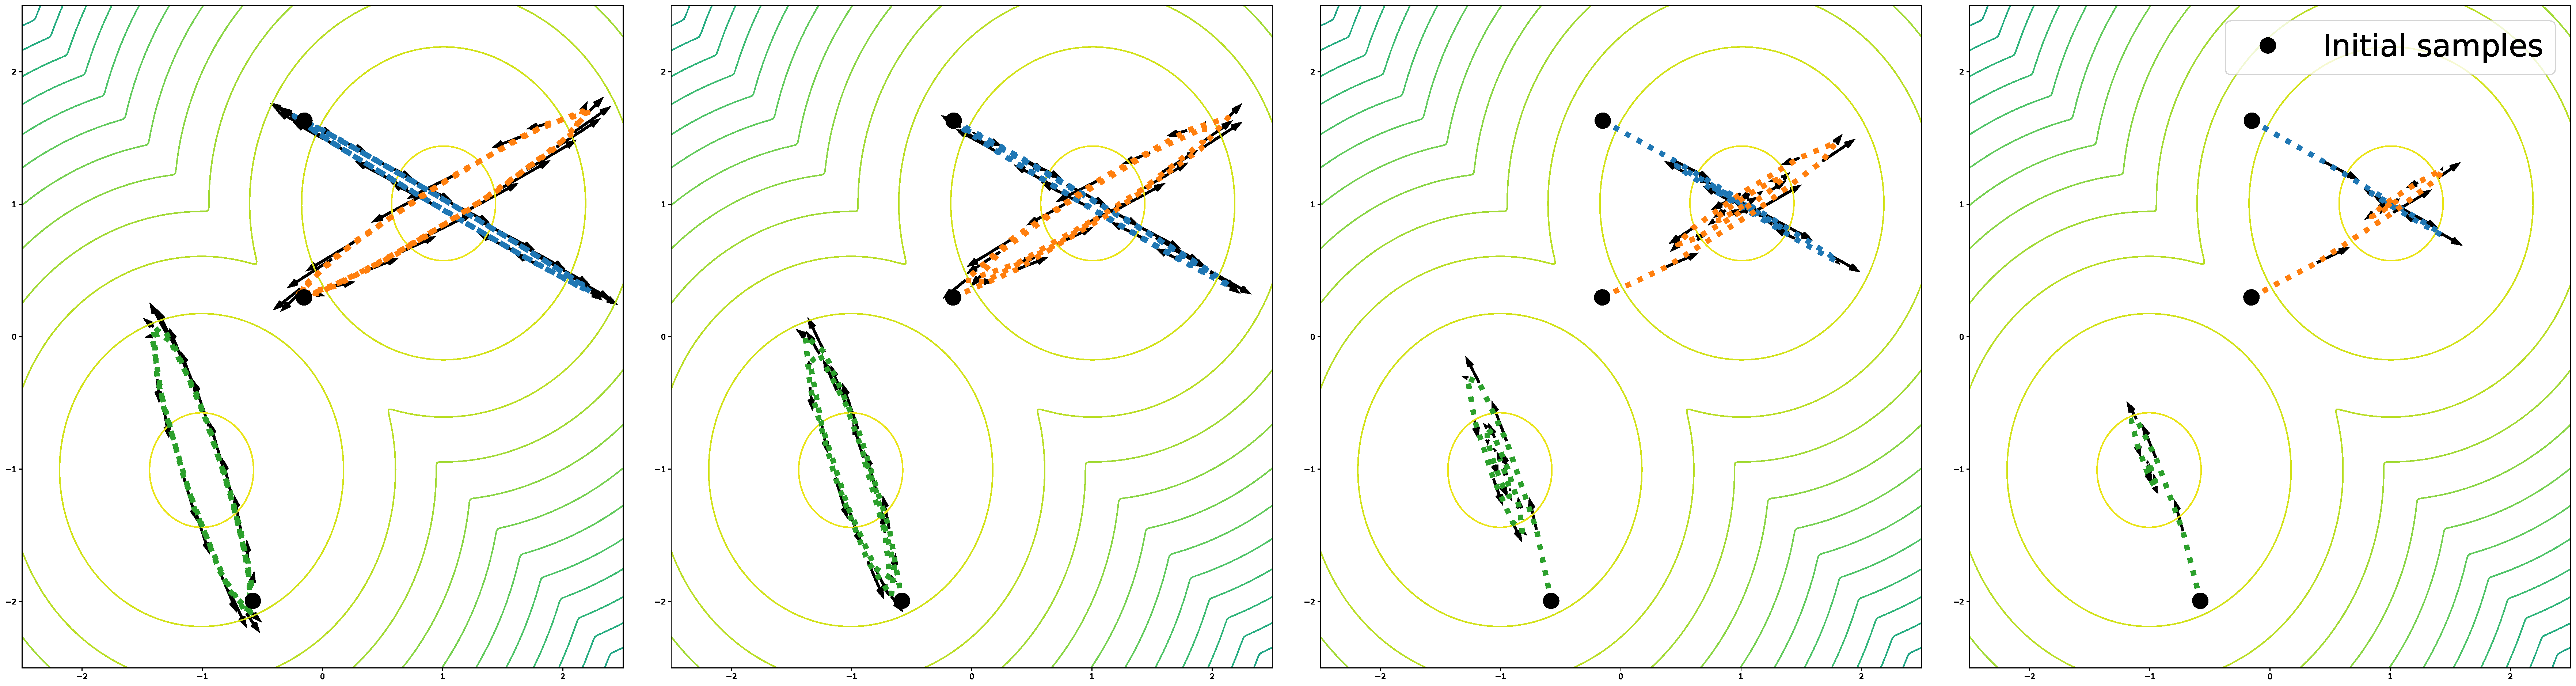
\includegraphics[width=1\linewidth]{bigplot.pdf}
\end{tabular}
     \caption{Conformal Hamiltonian paths for different values of the dissipation parameters for a mixture of two Gaussian distributions given different Hamiltonian parameters. From left to right, $\gamma$ increasing from 0 to 0.3, 2 and 4.}
     \label{fig:toy_example_posterior}
 \end{figure*}
In the applications below, we consider the conformal version of the symplectic Euler method of \eqref{eq:ODE_hamiltonian}, see \cite{francca2019conformal}.
This integrator can be constructed as a splitting of the two conformal and conservative parts of the system \eqref{eq:ODE_hamiltonian}. When composing a dissipative with a  symplectic operator, we set for all $(q,p) \in \rset^{2dn}$, $\transfo_h(q,p)$ to be
 \[
 (q+h\mass^{-1}\{ \rme^{-h\gamma} p -h \nabla U(q)\},
 \rme^{-h \gamma } p -h \nabla U(q))\eqsp,
\]
where $h >0$ is a discretization stepsize.
This transformation can be connected with classical momentum optimization schemes, see \cite[Section 4]{francca2019conformal}.
By \cite[Section 3]{francca2019conformal}, for any $h >0$ $\transfo_h$ is a $\rmC^1$-diffeomorphism on $\rset^{2d}$ with Jacobian given by $\JacOp{\transfo_h}(q,p) = \rme^{-\gamma h d}$. In addition,  its inverse is
$  \transfo_h^{
-1}(q,p) = (q-h\mass^{-1} p,\rme^{\gamma h}\{p+h \nabla U(q-h\mass^{-1} p)\})$.
Therefore, the weight \eqref{eq:def_w_k} of the  \IFIS\  estimator is given by
\begin{equation}
w_{k}(q,p) = \frac{ \tilde \rho(\transfo^k_h(q,p)) \rme^{-\gamma k h d} }{
    \sum_{j = k-K}^k  \tilde \rho(\transfo^j_h(q,p)) \rme^{-\gamma j h d} },
\end{equation}
where $\tilde \rho(q,p) \propto \rho(q) \rme^{-K(p)}$.
In the applications below, $\mass$ is chosen as a diagonal matrix with positive entries, see the  discussion  in \Cref{subsec:estim_constant}.

\section{InFiNE-based MCMC}\label{sec:infine:MCMC}
We describe here novel MCMC algorithms that leverage the $\InFiNE$ method to sample from $\pi$.

To motivate our sampler, let us recall the principle of the Sampling Importance Resampling method (SIR; \cite{rubin1987comment,smith1992bayesian}) whose goal is to approximately sample from the target distribution $\target$ using samples drawn from a proposal distribution $\proposal$.

In SIR, a $N$-\iid\ sample $\chunku{X}{1}{N}$ is first generated from the proposal distribution $\proposal$. A sample $X^*$ is approximately drawn from the target $\target$ by choosing randomly a value in $\chunku{X}{1}{N}$ with probabilities proportional to the importance weights $\{\weightfunc(X^i)\}_{i = 1}^N$, where $\weightfunc(x)= \target(x)/\proposal(x)$. Note that the importance weights are required to be known only up to a constant factor.  For SIR, as $N \to \infty$, the sample $X^*$ is \emph{asymptotically} distributed according to $\target$; see~\cite{smith1992bayesian}. Two major drawbacks of SIR are that it is only asymptotically valid and that the number $N$ of proposals should typically grow exponentially with the dimension $d$ of the state-space to maintain a given accuracy.

A subsequent algorithm  is the \emph{iterated SIR} (ISIR) \cite{andrieu2010particle}. In this version, the sample size $N$ is not necessarily large ($N\geq 2$), but the whole process of sampling a set of proposals, computing the importance weights, and picking a  candidate, is iterated. At the $n$-th step of ISIR, the active set of $N$ proposals $\chunku{X_n}{1}{N}$ and the index $I_n \in [N]$ of the conditioning proposal are kept. First ISIR  updates the active set  by setting $X_{n+1}^{I_n}= X_n^{I_n}$ (keep the conditioning proposal) and then draw independently $\chunkum{X_{n+1}}{1}{N}{I_n}$ from $\proposal$.
Then it selects the next proposal index $I_{n+1} \in [N]$ by sampling with probability
proportional to $\{\weightfunc(X_{n+1}^i)\}_{i=1}^N$.
As shown in \cite{andrieu2010particle}, this algorithm  defines  a partially collapsed Gibbs sampler (PCG) of the augmented distribution (see \Cref{subsec:ISIR-partially-collapsed-dependent})
$$
\bar{\measpi}(\chunku{x}{1}{N},i)=\frac{1}{N}  \target(x^i) \prod_{j \neq i} \proposal(x^j) =\frac{1}{N} \weightfunc(x^i) \prod_{j=1}^N \proposal(x^j) \eqsp.
$$
The PCG sampler can be shown to be ergodic provided that $\proposal$ and $\target$ are continuous and $\proposal$  is  positive on the support of $\target$. If in addition the importance weights are bounded, the Gibbs sampler can be shown to be uniformly geometrically ergodic  \cite{lindsten2015uniform,andrieu2018uniform}.
It follows that the distribution of the conditioning proposal $X_n^*= X_n^{I_n}$ converges to $\pi$ as the iteration index $n$ goes to infinity. Indeed, for any integrable function $f$ on $\rset^d$, with $(\chunk{X}{1}{N},I) \sim \bar{\measpi}$,
$$
\PE_{}[f(X^I)]= \int \sum_{i=1}^N f(x^i)  \bar{\measpi}(\chunku{x}{1}{N},i) \rmd \chunku{x}{1}{N} = N^{-1} \sum_{i=1}^N \int f(x^i) \target(x^i) \rmd x_i = \int f(x) \target(x) \rmd x \eqsp.
$$
When the state space dimension $d$ increases, designing a proposal distribution $\proposal$ guaranteeing proper mixing properties becomes more and more difficult. A way to circumvent this problem is to use dependent proposals, allowing in particular \emph{local moves} around the conditioning path. To implement this idea, for each $i \in [N]$, we define a proposal transition, $r_i(x^i; \chunkum{x}{1}{N}{i})$ which defines the the conditional distribution of $\chunkum{X}{1}{N}{i}$ given  $X^i= x^i$. The key property validating ISIR with dependent proposals (see \Cref{subsec:ISIR-partially-collapsed-dependent}) is that all one-dimensional marginal distributions are equal to $\proposal$, which requires that for each $i,j  \in [N]$,
\begin{equation}
\label{eq:conditional-decomposition}
\proposal(x^i) r_i(x^i;\chunkum{x}{1}{N}{i})=
\proposal(x^j) r_j(x^{j};\chunkum{x}{1}{N}{j})
\end{equation}
The (unconditional) joint distribution of the particles is therefore defined as
\begin{equation}
\label{eq:joint-distribution}
\proposal_N\bigl(\chunku{x}{1}{N}\bigr) = \proposal(x^1) r_1(x^1;\chunkum{x}{1}{N}{1}) \eqsp.
\end{equation}
The resulting modification of the ISIR algorithm is straightforward: $\chunkum{X}{1}{N}{I_n}$ is sampled jointly from the conditional distribution $r_{I_n}(X_n^{I_n},\cdot)$ rather than independently from $\proposal$.

There are many ways to make proposals dependent. For instance, dependence may be induced by using a Markov kernel reversible \wrt\ to the proposal $\proposal$, i.e., such that $\proposal(x) m(x,x')= \proposal(x') m(x',x)$, assuming for simplicity that this kernel has density $m(x,x')$ \cite{ruiz:titsias:doucet:2020}. In this case, for each $i \in [N]$, the conditional proposal kernel is
\begin{equation}
\label{eq:condition-kernel}
r_i(x^i,\chunkum{x}{1}{N}{i})  =\prod_{j=1}^{i-1} m(x^{j+1},x^{j}) \prod_{j=i+1}^n m(x^{j-1},x^j) \eqsp.
\end{equation}
A straightforward induction shows that \eqref{eq:conditional-decomposition} is satisfied and that the joint distribution of the particles (see \eqref{eq:joint-distribution} is given by  $\proposal_N(\chunku{x}{1}{N})=\proposal(x^i) \prod_{j=2}^{N} m(x^{j-1},x^j)$. If $\proposal$ is Gaussian, an appropriate choice is an autoregressive kernel $m(x,x')= \phi_d(x';\alpha x, \sqrt{1-\alpha^2} \Id_d)$, where $\phi_d(x; \mu, \Sigma)$ is the $d$-dimensional Gaussian pdf with mean $\mu$ and covariance $\Sigma$ as in  \cite{ruiz:titsias:doucet:2020}. More generally, we can use a Metropolis-Hastings kernel with invariant distribution $\proposal$.

 We now propose the \IFIS\ MCMC sampler which extends the ISIR algorithm to \IFIS\ construction.  The input for the $n$-th iteration comprises an active set  of $N$ path initial states,  $\chunku{X}{1}{N}$, the index $1\le I_n\le N$ of the conditioning path, and the iteration index $0\le K_n\le K$ along the conditioning path.
Adopting the ISIR protocol, our sampler proceeds as follows.
\begin{enumerate}
\item Set  $X_{n+1}^{I_n}= X_n^{I_n}$ and draw the remaining proposals $\chunkum{X_{n+1}}{1}{N}{I_{n}} \sim r_{I_n}(X^{I_n},\cdot)$.
\item For each initial value $X_{n+1}^i$, $i \in [N]$, compute the iterates $\{ \transfo^k(X_{n+1}^i) \}_{k=1}^K$.
\item Draw the path index $I_{n+1}  \in [N]$  with probability proportional to  $(\estConstC{X_{n+1}^{i}})_{i \in [N]}$, with $\estConstC{X_{n+1}^{i}}$ defined in  \eqref{eq:def_estimator_normal_const_1}.
\item Draw the next iteration  index $0\le K_{n+1} \le K$ on the conditioning path with probability proportional to
\[
\w_k(X^{I_{n+1}}_{n+1})\likelihood(\transfo^k(X^{I_{n+1}}_{n+1})) \eqsp.
\]
\end{enumerate}
Similar to ISIR, \IFIS\ MCMC is a partially collapsed Gibbs sampler targeting the extended pdf (see \Cref{subsec:partial-collapsed-infine}) 
\begin{align}\label{eq:def_measpi_N}
\nonumber
&  \bar{\measpi}(x^{1:N},i,k) \\
\nonumber
  &= {\w_k(x^i)\likelihood(\transfo^{k}(x^i) \proposal(x^i) r_i(x^i;\chunkum{x}{1}{N}{i})}\big/{N \const} \\
  &= {\w_k(x^i)\likelihood(\transfo^{k}(x^i)
  )}\proposal_N(\chunku{x}{1}{N})\big/{N \const}
   \eqsp.
\end{align}
whose marginal distribution satisfies
\[
\bar{\measpi}(\chunku{x}{1}{N},i)=\frac{1}{N \const}  \estConstC{x^i} \proposal(x^i) r_i(x^i;\chunkum{x}{1}{N}{i})\eqsp.
\]
Under mild conditions (see \Cref{sup:sec:ergodicity}), this PCG sampler is ergodic, hence the distributions of the iterates $(\chunku{X_n}{1}{N},I_n,K_n)$ and of their projections $X^*_n=\transfo^{K_{n}}(X_n^{I_n})$ converge to $\bar{\measpi}$ and to $\target$, respectively. Indeed, for any integrable function $f$ on $\rset^d$, with $(\chunk{X}{1}{N},I,K)\sim \bar{\measpi}$,
 \begin{align*}
    & \PE[f(T^K(X^I))]= \sum_{i=1}^N\int_{}\sum_{k=0}^K\bar{\measpi}(x^{1:N},i,k)f(T^k(x^i))
    \rmd \chunku{x}{1}{N}  \\
    &=(N \const)^{-1}\! \sum_{i=1}^N\!\int_{}\sum_{k=0}^K   \rho(x^i) \w_k(x^i)  \likelihood(\transfo^{k}(x^i))f(\transfo^k(x^i)) \rmd x^i
    \\
    & = (N \const)^{-1} \sum_{i=1}^N\int_{} \rho(x^i) \likelihood(x^i)f(x^i) \rmd x^i = \int_{} \measpi(y)f(y) \rmd y \eqsp,
\end{align*}
following \Cref{theo:inf_non_eq}.
%\end{proof}
The \IFIS\  MCMC sampler is thus a valid procedure to generate samples from $\measpi$. When the transformation $\transfo$ is chosen as in \Cref{subsec:NISestimators}, our sampler draws samples based on optimization paths. Detailed experiments are discussed in \Cref{subsec:mcmc_exp}.



\section{ELBO for variational auto-encoders}
\label{sec:extensions}
\begin{comment}
For high dimensional observations $y$, Variational Auto-Encoders (VAE)  build upon some latent variables $x\in\rset^d$ to define a likelihood model as
\begin{equation}\label{eq:demarge}
p_\theta(y) = \int p_\theta(y\mid x) p(x) \rmd x = \int p_\theta(x,y) \rmd x\eqsp.
\end{equation}
As this integral representation is not tractable, and approximating it naively by Monte Carlo would result in a large variance, \cite{kingma:welling:2013} introduced a parametric family of distributions $\{q_\phi(\cdot\mid y)\}_\phi$ approximating $p_\theta(\cdot\mid y)$.
\end{comment}
Given a joint model $p_\theta(y, x)$, with data $y \in \rset^p$ and latent variable $x \in \rset^d$, variational inference (VI)
provides us with a tool to both approximate the intractable
posterior $p_\theta(x|y)$ and maximize the marginal likelihood
$p_\theta(y)= \int p_\theta(x,y) \rmd x$ in the parameter $\theta$. This is achieved by introducing a
parameterized approximate posterior $q_\phi(x|y)$ and maximizing
the Evidence Lower Bound (ELBO) (see \cite{kingma2019introduction})
\begin{align}\label{eq:elbo}
\mathcal{L}_{\textup{ELBO}}(\theta,\phi)&= \int \log\left(\frac{p_\theta(x,y)}{q_\phi(x\mid y)}\right) q_\phi(x\mid y)\rmd x \eqsp\\
&=\log p_\theta(y)-\operatorname{KL}(q_\phi(\cdot\mid y) \| p_\theta(\cdot\mid y) )\eqsp,\nonumber
\end{align}
where $\operatorname{KL}$ is the Kullback–Leibler divergence.
Towards more flexibility, approximate posteriors can be defined as marginal distributions, $q_\phi(x|y) = \int
\bar{q}_\phi (x, u |y) \rmd u$, where $u \in \mathsf{U}$ is an auxiliary variable (which can both have discrete ann dontinuous components) and $\bar{q}_\phi(x,u|y)$ is a generative closed-form density. 
Introducing auxiliary variables loses the tractability of \eqref{eq:elbo} but they allow for their own ELBO as suggested in \cite{agakov2004auxiliary}; \cite{lawson2019energy}, leading to the objective
\begin{equation}\label{eq:AVI_ELBO}
\int \bar{q}_\phi(x,u|y) \log \left( \frac{\bar{p}_\theta(x,u,y)}{\bar{q}_\phi(x,u|y)} \right)  \rmd x \rmd u \eqsp,
\end{equation}
where $\bar{p}_\theta(x,u,y)$ is an extended joint likelihood satisfying $p_\theta(x,y)= \int \bar{p}_\theta(x,u,y) \rmd u$ (or equivalently $\bar{p}_\theta(x,u,y)= p_\theta(x,y) \bar{m}_\theta(x,y; u)$ where $\bar{m}_\theta(x,y;\cdot)$ is a Markov kernel).
We now exploit this idea within the \IFIS\ framework. For that purpose, set prior, likelihood, and posterior as $\proposal(x)=q_\phi(x\mid y)$, $\likelihood(x)= p_\theta(x,y)/ q_\phi(x \mid y)$, and $\target(x)=p_{\theta}(x\mid y)$, respectively (the dependence of $\proposal$, $\likelihood$, and $\target$ on both parameter $(\theta$, $\phi)$ and observation $y$ is implicit for notational simplicity). With these notations, the normalizing constant of $\proposal(x) \likelihood(x)$ is then  $\const= p_\theta(y)$. The auxiliary variable $u$ is naturally associated with the extended target $\bar{\measpi}$ defined in \eqref{eq:def_measpi_N} (playing the role of $\bar{p}_\theta$), with
$$
(x,u)=([x,\chunkum{x}{1}{N}{i}],i,k)\eqsp,
$$
$[x,\chunkum{x}{1}{N}{i}]$ being a shorthand notation for a $N$-tuple $\chunku{x}{1}{N}$ with $x^i= x$. An extended proposal playing the role of $ \bar{q}_\phi(x,u|y)$ is derived from the \IFIS~MCMC sampler, i.e.
\begin{equation}
\label{eq:proposal-extended}
\bar{\proposal}(\chunku{x}{1}{N},i,k)=  \frac{\likelihood(\transfo^k(x^i)) \w_k(x^i)}{N \estConstC{\chunku{x}{1}{N}}} \proposal_N(\chunk{x}{1}{N})  \eqsp.
\end{equation}
where $\estConstC{\chunku{x}{1}{N}}$ is the \IFIS\ estimator \eqref{eq:def_estimator_normal_const} of the normalizing constant.
Note that, by construction, 
\begin{equation}
\label{eq:expression-marginal}
\sum_{i=1}^N \sum_{k=0}^K \bar{\proposal}(\chunku{x}{1}{N},i,k) = \proposal_N(\chunku{x}{1}{N})
\end{equation}
showing that this joint proposal can be sampled by drawing the proposals $\chunku{x}{1}{N} \sim \rho_N$, then sampling the path index $i \in [N]$ with probability proportional to $(\estConstC{x^i})_{i=1}^N$ (with $\estConstC{x}$ defined in \eqref{eq:def_estimator_normal_const_1}) and finally the iteration index $k \in \{0,\dots,K\}$ with probability proportional to $(\w_k(x^{i})\likelihood(\transfo^k(x^{i}))_{k=0}^K$.
\begin{comment}
this lower bound can be inaccurate. To improve it, we can exploit any unbiased positive estimate $\hat{p}_{\theta}(y)$ of the marginal likelihood.
Indeed $\log p_\theta(y)= \log \mathbb{E}[\hat{p}_{\theta}(y)]\geq \mathbb{E}[\log \hat{p}_{\theta}(y)]$ by Jensen's inequality.
\cite{mnih2016variational} argue that the better the estimator $\hat{p}_\theta(y)$, the better the ELBO.
\end{comment}
Since the ratio of \eqref{eq:def_measpi_N} over \eqref{eq:proposal-extended} is
\begin{equation}
\label{eq:ratio-extended}
{\bar{\measpi}(\chunku{x}{1}{N},i,k)}\big/{\bar{\proposal}(\chunku{x}{1}{N},i,k)}= {\estConstC{\chunku{x}{1}{N}}}\big/{\const} \eqsp.
\end{equation}
The augmented ELBO   \eqref{eq:AVI_ELBO} writes
\begin{align}
 \label{eq:infine_elbo-alt}
\elboneq &= \int_{} \proposal_N( \chunku{x}{1}{N})   \log \estConstC{\chunku{x}{1}{N}} \rmd \chunku{x}{1}{N}\eqsp,\\
\nonumber
 &=  \log \const - \operatorname{KL}( \bar{\proposal} | \bar{\measpi} )\eqsp,
\end{align}
where we have used \eqref{eq:expression-marginal} and that the ratio ${\bar{\measpi}(\chunku{x}{1}{N},i,k)}\big/{\bar{\proposal}(\chunku{x}{1}{N},i,k)}$ does not depend on 
the path index $i$ and the proposal index $k$ along the path. When $K=0$ and $\proposal_N(\chunku{x}{1}{N})= \prod{j=1}^N \proposal(x^j)$, we exactly retrieve the Importance Weighted AutoEncoder (IWAE); see e.g.  \cite{burda:grosse:2015} and in particular the interpretation in \cite{cremer2017reinterpreting}. 

Choosing the conformal Hamiltonian introduced in \Cref{subsec:NISestimators} allows for a family of invertible flows that depends on the parameter $\theta$ which itself is directly linked to the target distribution.


\section{Numerical Experiments}
\subsection{Normalizing constant estimation}
\label{subsec:estim_constant}
We first consider the problem of the estimation of the normalizing constant of Gaussian mixtures in dimension $d$ in two different settings. In the first experiment, we consider an (unnormalized)  mixture of two Gaussian distributions, with equal mixing weights. The mean of the two components are set to $(\mathbf{1}_d, -\mathbf{1}_d)$, where $\mathbf{1}= [1,\dots,1]^T$ and covariance $\sigma ^2 \Id = 0.02$.
The second target is an unnormalized mixture of 25 $d$-dimensional Gaussian distributions in dimension $d=10,20$. Each component has the same covariance assumed to be diagonal with diagonal elements equal to $(0.01,0.01, 0.1, \ldots, 0.1)$. The means are given by $(i,j,0,\ldots,0)$ with $i,j \in \{-2,\ldots, 2\}$, see \Cref{fig:25_gauss_mcmc}.  The normalizing constant in this case is 12.5. In both examples the proposal $\rho$ is chosen to be a $d$-dimensional Gaussian, with zero mean and diagonal covariance $\sigma^2_\proposal \Id_d$, with $\sigma^2_\rho=5$. 
The performance of the $\IFIS$ estimator \eqref{eq:def_estimator_normal_const} is first illustrated in this toy problem for $d\in\{5,10,15,20\}$ and different choices of parameters.

Our approach is compared with a na{\"\i}ve IS estimator using the same proposal $\rho$. 
A state-of-the-art competitor for the estimation of normalizing constants, the AIS estimator of \cite{neal:2001,tokdar2010importance} is also included in the comparison.
AIS relies on a sequence of target distribution $\target_k(x)$, $0 \leq k \leq K$ with $\target_0(x)= \proposal(x)$ and $\target_K(x)= \target(x)$. AIS defines an extended target and proposal using MCMC kernels which are reversible for each linking densities $\target_k$; most often, these MCMC kernels use Langevin or Hamiltonian dynamics; see \eg\ \cite{buchholz2021adaptive}. Therefore, AIS is directly comparable to the \IFIS\ estimator in terms of complexity.
\begin{figure}[!ht]
    \centering
    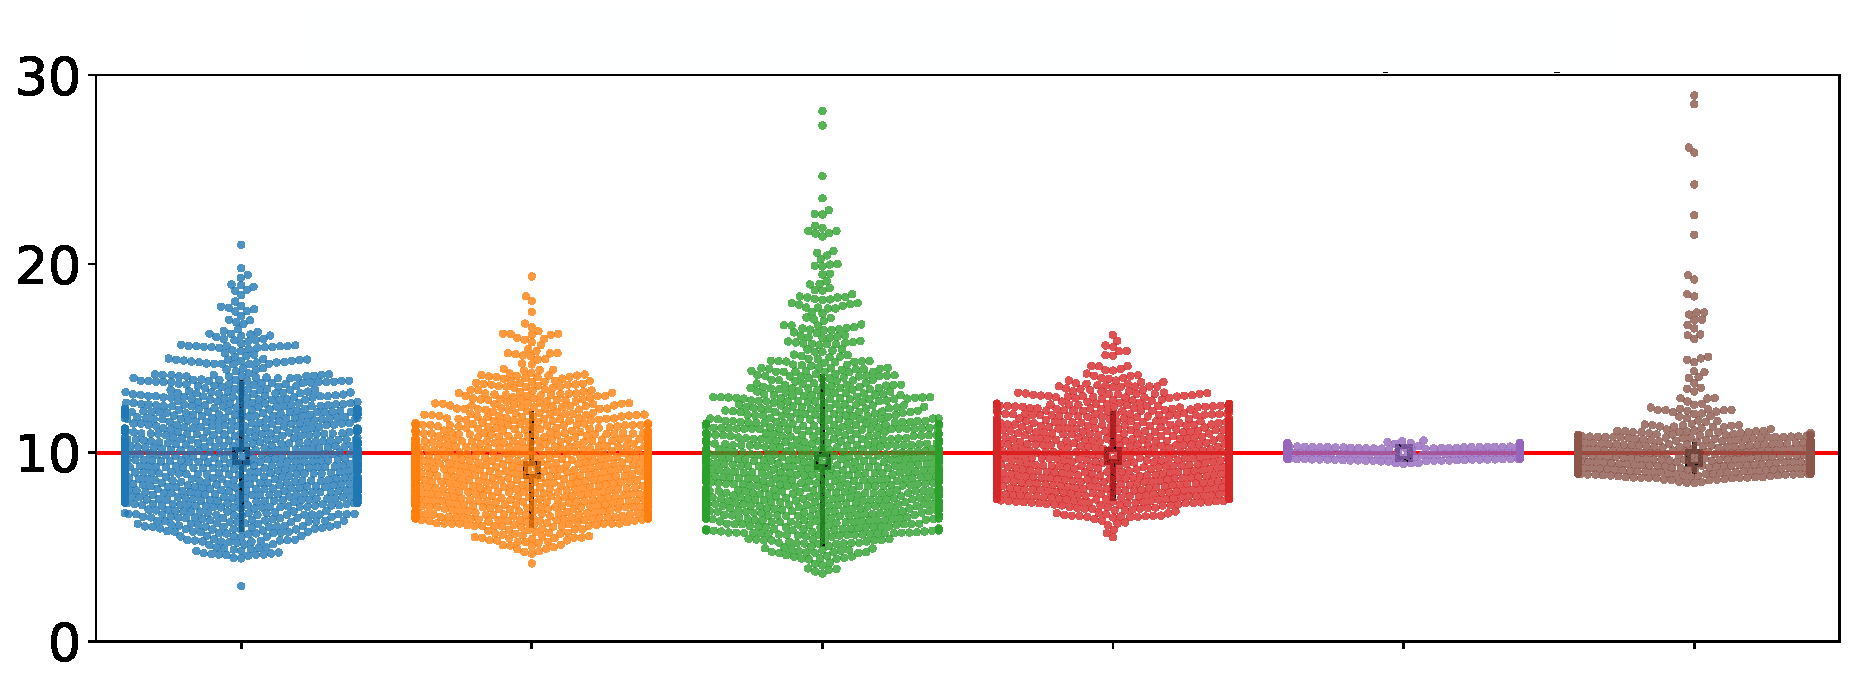
\includegraphics[width= \linewidth]{boxplot_two_gaussian_dim_5.pdf}
    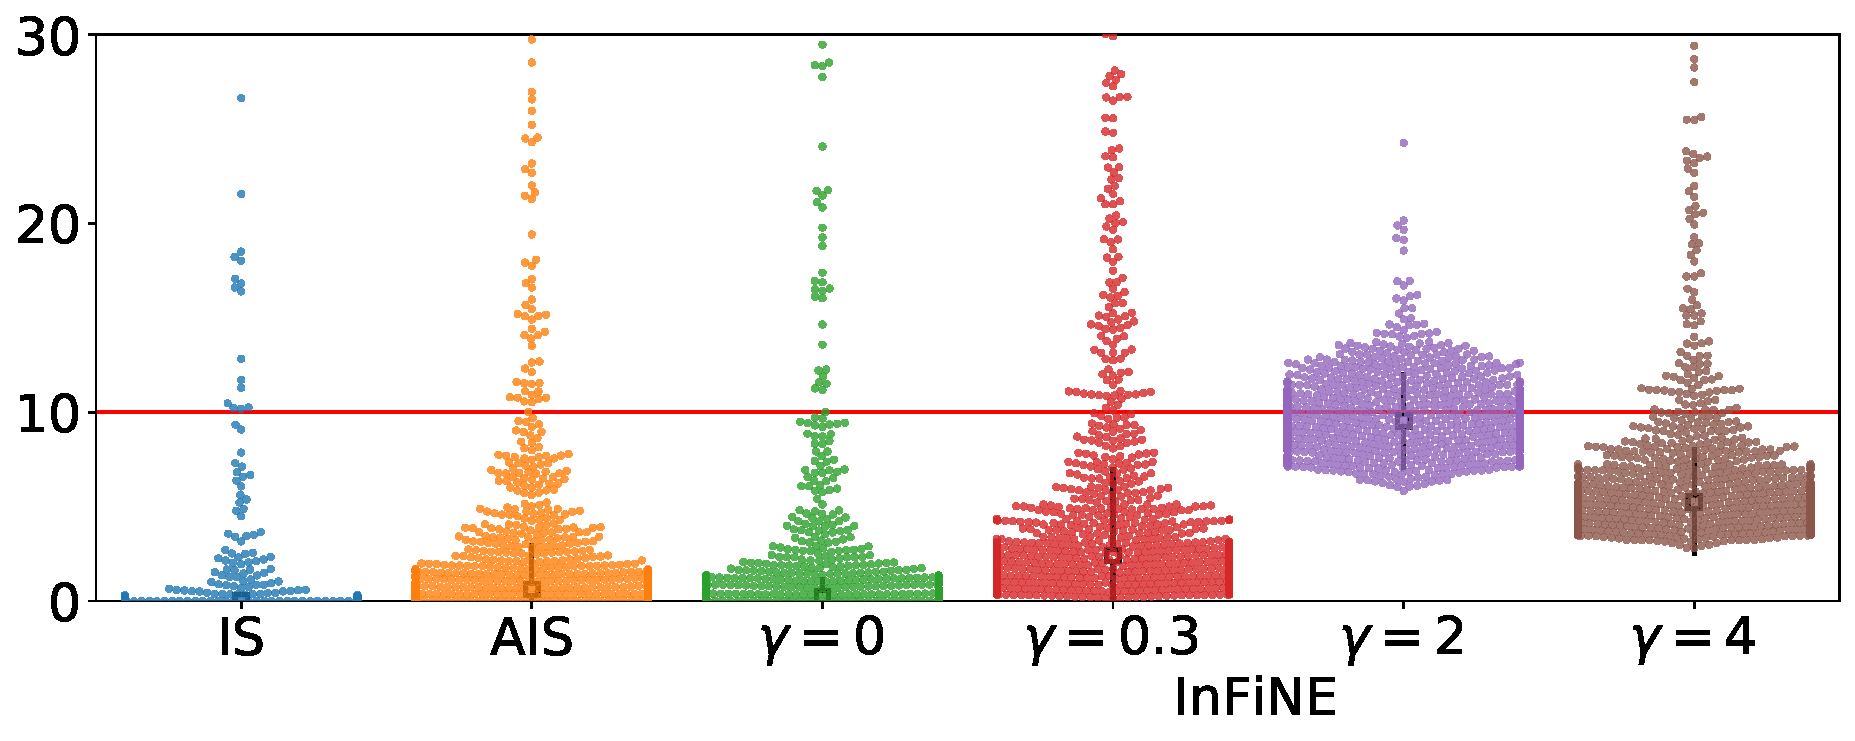
\includegraphics[width= \linewidth]{boxplot_two_gaussian_dim_10.pdf}
    \caption{1000 independent estimations of the normalizing constant for each algorithm in the toy example:  a mixture of two Gaussian distributions, in dimension 5 (top) and 10 (bottom). The true value is $Z=10$ (red line). The figure displays the median (square) and the interquartile range (solid lines) in each case.}
    \label{fig:simple_gauss}
\end{figure}
We focus here on the impact of the damping factor $\gamma$ on the $\IFIS$ estimations. Further investigation on the stepsize $h$ and of the mass matrix $\mass$  are given in the supplementary material.

The number of steps $K$ is  a proxy of our computational budget (\ie~the number of times our transformation is applied). The mass matrix $\mass$ is chosen as the inverse of the covariance of the individual component of the mixture. Further tuning on this matrix is discussed in the supplementary material.
A first intuition on the role of $\gamma$ is shown in \Cref{fig:toy_example_posterior}. If $\gamma \ll 1$, then the trajectories are almost Hamiltonian, in which case we cannot easily explore all modes. On the other hand, if $\gamma \gg 1 $,  then trajectories are most often attracted by the ``closest'' mode. The resulting trade-off is easily observed on \Cref{fig:simple_gauss}, which displays the distribution of the different estimators.


The IS estimator is run with $4 \cdot 10^5$ samples.
For the \IFIS\ estimator, the number of samples is $N = 2 \cdot 10^4$ and the trajectory length is $K=20$. The stepsize is set to $h= 0.1$ for the conformal symplectic integrator.
The number of levels for AIS in the annealing schedule of AIS is set to $200$. At each intermediate temperature, an iteration of HMC is performed with 3 leapfrog steps (the size of leapfrog step is also set to 0.1).
The number of gradient computations is therefore equal to $4 \cdot 10^5$ for \IFIS\ and $6 \cdot 10^6$ for AIS, which is therefore 10 times more costly.

We further emphasize how the \IFIS\ estimator compares favorably to the AIS estimator albeit requiring a smaller computational budget.
\begin{figure}[!ht]
    \centering
    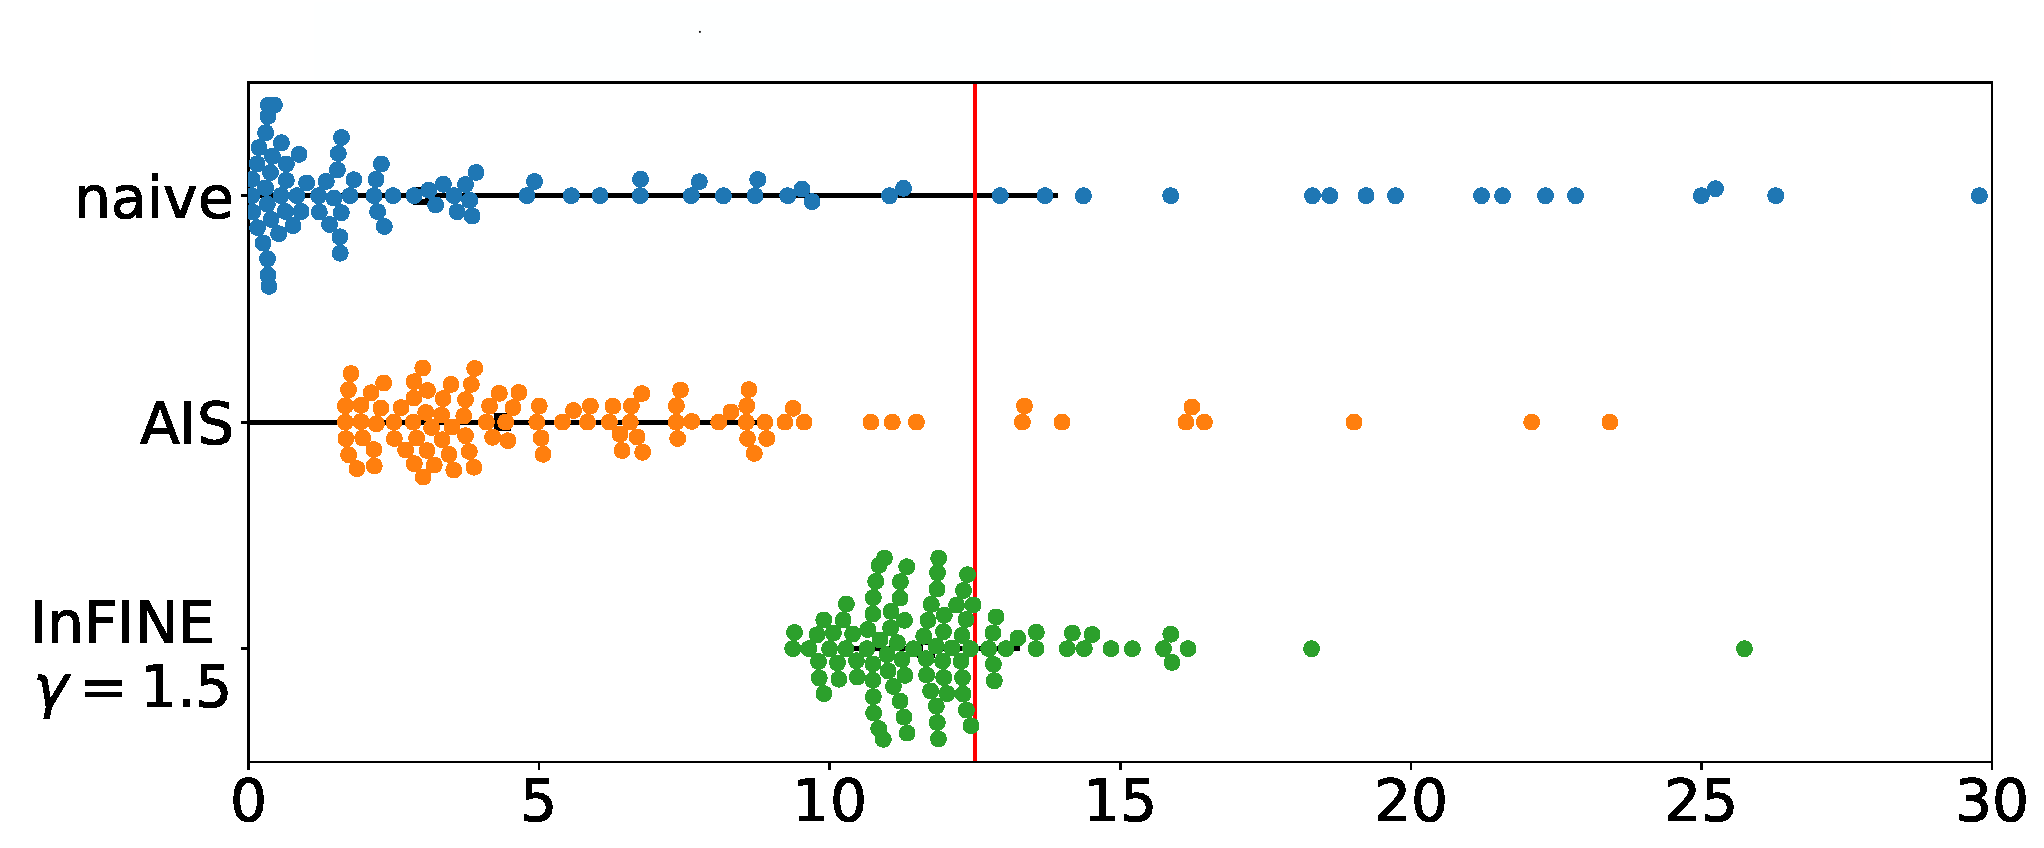
\includegraphics[width= 1.\linewidth]{boxplot_dim10.pdf}
        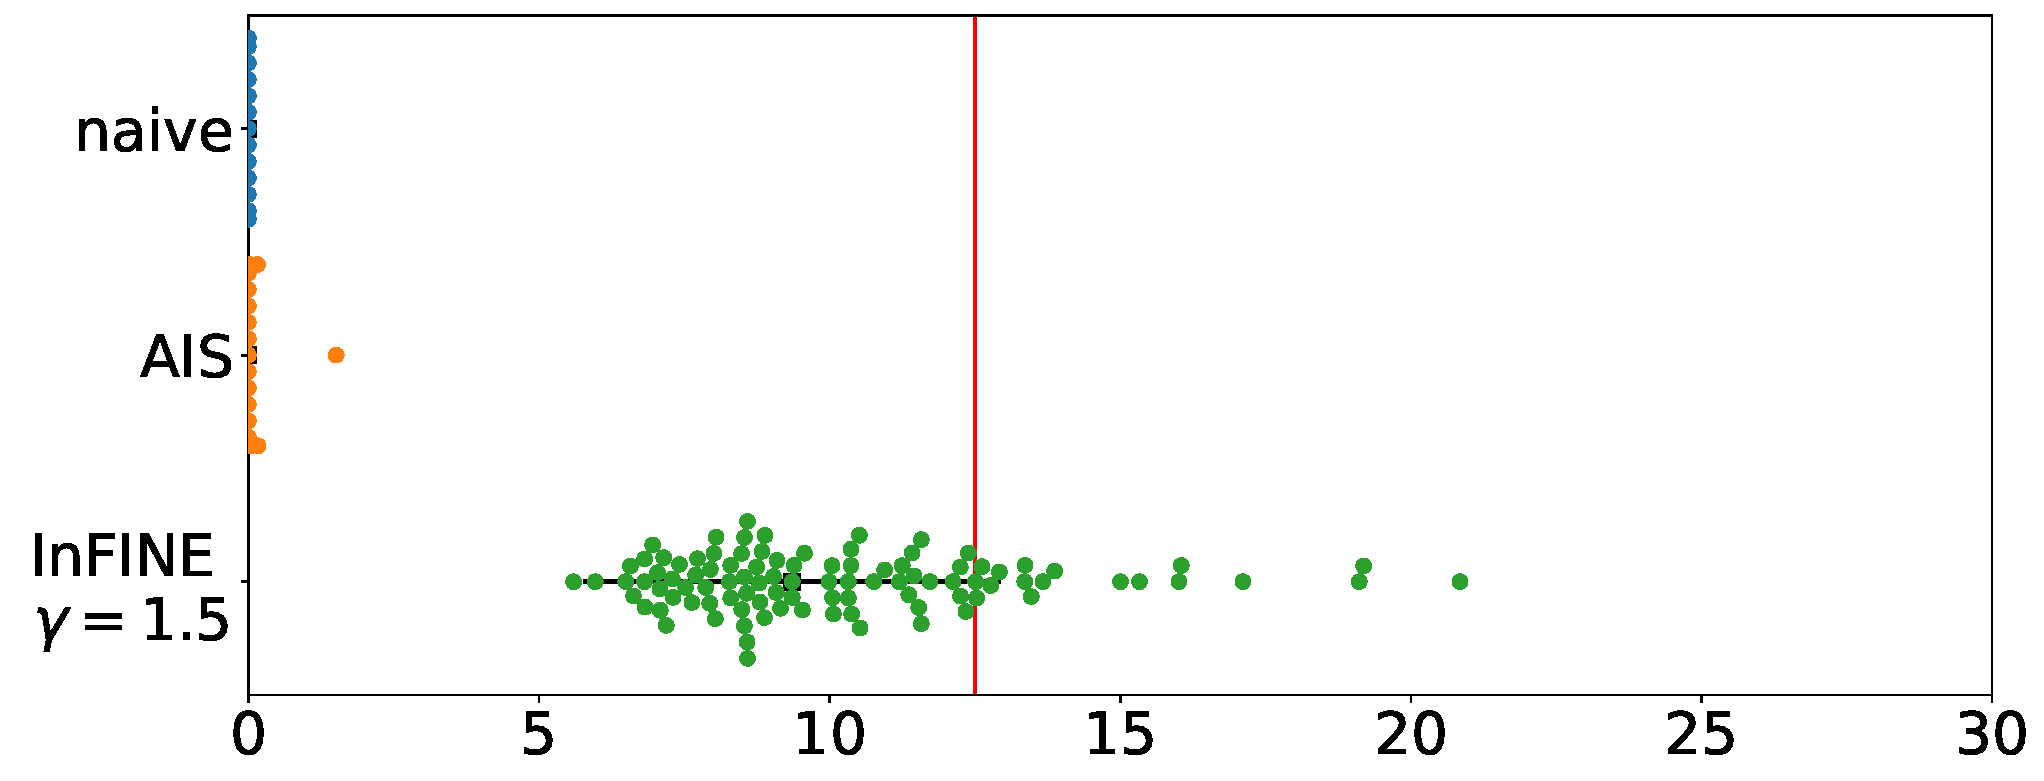
\includegraphics[width= 1.\linewidth]{boxplot_dim20.pdf}
    \caption{$100$ independent estimations of the normalizing constant of the Gaussian mixture with 25 components in dimension 10 (top) and 20 (bottom) for each algorithm. The true value is $Z=12.5$ (red line).}
    \label{fig:25_gauss}
\end{figure}

The results for the 25-component Gaussian mixture are displayed in \Cref{fig:25_gauss}. In high dimension, the vanilla IS estimator unsurprisingly fails, since importance weighted estimates have notoriously poor scaling properties w.r.t. dimension. While AIS predictably improves upon vanilla IS, its performances are rather unsatisfactory, the estimator showing a very large variance. Regardless of the dimension $d$, the \IFIS\ estimator  is better behaved than the AIS estimator, although the computational burden for \IFIS\ is 10 times smaller.
\begin{comment}
\begin{table}[]
\caption{Results for the estimation of the normalizing constant in the toy example:  a mixture of two peaked Gaussians, in dimension 5. The true value is $Z=1$.}
\label{tab:simple_gaussian_est}
\begin{tabular}{c|c|c|}
\cline{2-3}
                                                 & Mean & Standard deviation \\ \hline
\multicolumn{1}{|c|}{IS estimate}                &    $6\cdot10^{-5}$  &           $6\cdot10^{-4}$         \\ \hline
\multicolumn{1}{|l|}{AIS estimate}               &  $3\cdot10^{-3}$    &    $2\cdot10^{-2}$                \\ \hline
\multicolumn{1}{|l|}{$\IFIS$ - $\gamma=0$}   &   $0.49$   &      4.9              \\ \hline
\multicolumn{1}{|l|}{$\IFIS$ - $\gamma=1$} &  $0.45$    &          2.5          \\ \hline
\multicolumn{1}{|l|}{$\IFIS$ - $\gamma=3$}   &   0.93   &   0.31                 \\ \hline
\multicolumn{1}{|l|}{$\IFIS$ - $\gamma=6$}   &  1.0    &        0.64            \\ \hline
\end{tabular}
\end{table}
\end{comment}
\subsection{MCMC experiments}
\label{subsec:mcmc_exp}
We focus here on sampling of the 25 Gaussian mixture example introduced in \Cref{subsec:estim_constant}. The dimension is set to $d=40$  and all the mixture components have diagonal covariances  $0.01 \Id_d$.
We compare the \InFiNE\ MCMC sampler with dependent proposals,
the No-U-Turn Sampler implemented with Pyro library \cite{bingham2019pyro},
and the ISIR scheme \cite{andrieu2010particle, andrieu2018uniform}, with correlated proposal.

For the \InFiNE\ MCMC, the number of particles is set to $N=10$, the length of trajectory is $K=10$, the stepsize of the conformal integrator is $h=0.1$, the mass matrix is diagonal with diagonal elements equal to 100. The proposal distribution is zero-mean Gaussian with diagonal covariance $5 \Id_d$. We use the proposal kernels $r_i$ defined in \eqref{eq:condition-kernel} with a random walk Metropolis kernel $m$ with zero-mean Gaussian increment distribution and covariance $0.01 \Id$.
For the iterated ISIR, we use the same number of proposals $N=10$,  proposal distribution $\proposal$ and proposal kernels $r_i$ as for \IFIS.  For NUTS, we use the default parameter (the mass matrix and stepsizes are adapted).

In \Cref{fig:25_gauss_mcmc}, the scatter plot of the first two components of the output is displayed. To make a fair comparison, we use the same wall clock time for all three algorithms. The number of iterations for CISIR, \IFIS, and NUTS are $n= 4\cdot 10^6$, $n= 4 \cdot 10^5$, and $n= 5 \cdot 10^5$, respectively.
\begin{figure}[!ht]
    \centering
    \begin{tabular}{cc}
      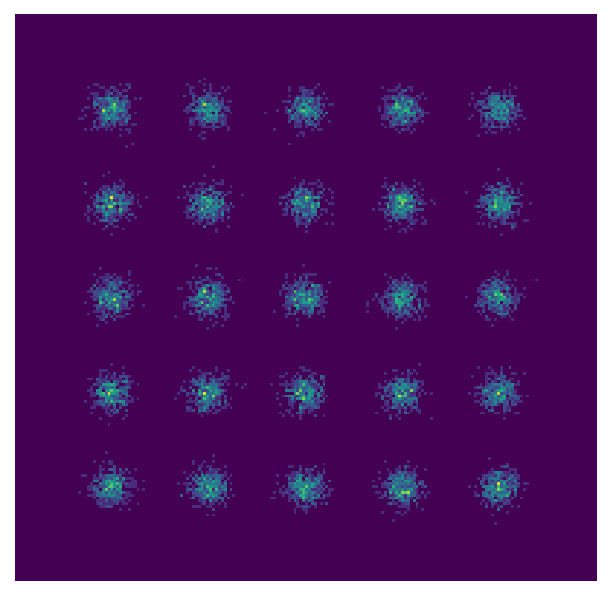
\includegraphics[width = .4\linewidth]{histogram_true.pdf}
      &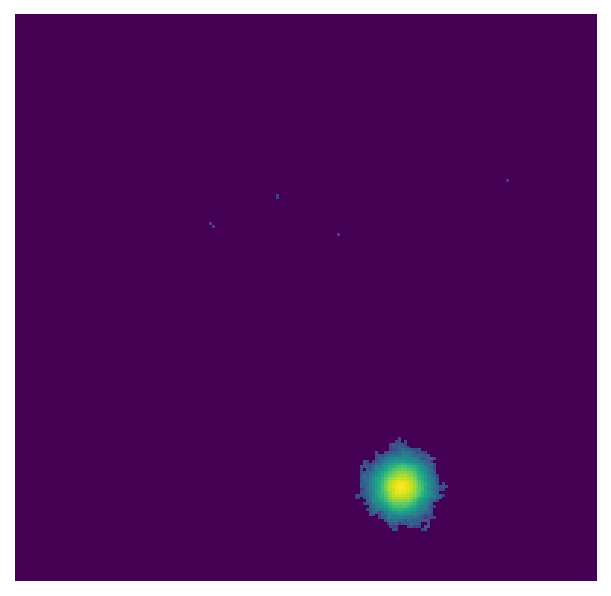
\includegraphics[width = .4\linewidth]{histogram_isir.pdf}  \\
       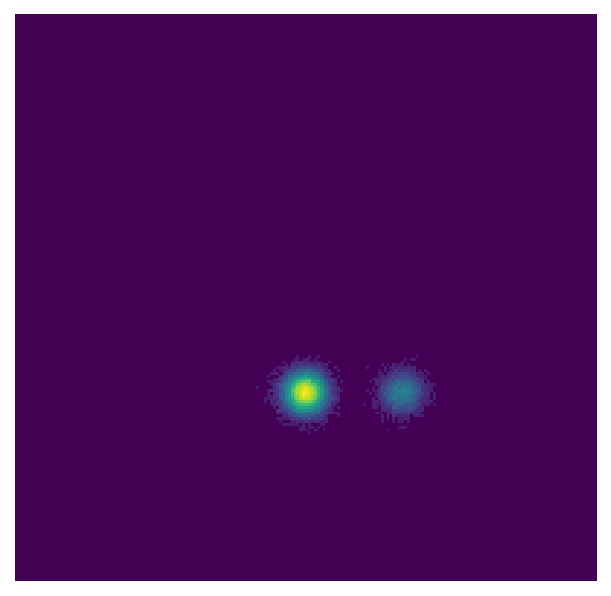
\includegraphics[width = .4\linewidth]{histogram_nuts.pdf}
       &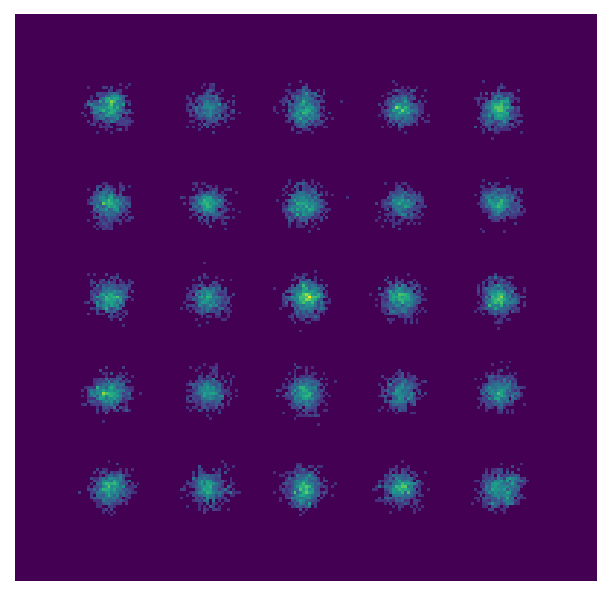
\includegraphics[width = .4\linewidth]{histogram_infine.pdf}
    \end{tabular}
    \caption{Empirical 2-D histogram of the 10,000 samples of different algorithms targeting the mixture of 25 Gaussian distributions. Top row, from left to right: samples from the target distribution, correlated ISIR samples. Bottom row: NUTS samples, \InFiNE\ samples.}
    \label{fig:25_gauss_mcmc}
\end{figure}
\begin{table*}[!t]
\centering
\caption{Negative Log Likelihood estimates for VAE models for different latent space dimensions.}
\label{tab:vae_results2}
\begin{tabular}{c|c|c||c|c||c|c||c|c|}
\cline{2-9}
 & \multicolumn{2}{c||}{$d = 4$} & \multicolumn{2}{c||}{$d = 8$} & \multicolumn{2}{c||}{$d = 16$} & \multicolumn{2}{c|}{$d = 50$} \\ \hline
\multicolumn{1}{|c|}{model} & IS & \InFiNE  & IS & \InFiNE& IS  & \InFiNE & IS & \InFiNE \\ \hline
\multicolumn{1}{|c|}{VAE} & $115.01$&$113.49$&$97.96$&$97.64$&$90.52$&$90.42$&$88.22$&$88.36$\\ %\hline
\multicolumn{1}{|c|}{IWAE, $N=5$} & $113.33$&$111.83$&$97.19$&$96.61$&$89.34$&$89.05$&$87.49$&$87.27$ \\ %\hline
\multicolumn{1}{|c|}{IWAE, $N=30$} & $111.92$&$110.36$&$96.81$&$95.94$&$88.99$&$88.64$&$86.97$&$86.93$ \\ \hline
\multicolumn{1}{|c|}{\InFiNE\ VAE, $K=3$} & $109.14$&$107.47$&$94.50$&$94.26$&$89.03$&$88.92$&$88.14$&$88.16$ \\ %\hline
\multicolumn{1}{|c|}{\InFiNE\ VAE, $K=10$} & $110.02$&$107.90$&$94.63$&$94.22$&$89.71$&$88.68$&$88.25$&$86.95$ \\ \hline
\end{tabular}
\end{table*}

\subsection{VAE experiments}
\label{subsec:vae_experiments}
 Following \Cref{sec:extensions}, we propose numerical experiments to illustrate the relevance of  \IFIS\ in the context of VAEs. We build \IFIS\ VAE by optimizing directly the ELBO \eqref{eq:infine_elbo-alt} with respect to the parameters $(\theta, \phi)$ with a single trajectory. In practice, extending a standard VAE implementation with \IFIS\ is straightforward: after sampling the initial position $q$ from the encoder distribution $q_\phi(\cdot\mid x)$, an initial moment $p$ is sampled. The trajectory is then computed, followed by the weights and the ELBO.
The \textit{reparameterization trick} \cite{kingma:welling:2013} is used in a similar fashion as the VAE to ensure full differentiability of the whole architecture, enabling the optimization of all parameters. A full specification of the algorithm is provided in \Cref{subsec:vae_algo}.

We follow the experimental setting of \cite{burda:grosse:2015}, using the MNIST dataset. Additional experiments on the FashionMNIST dataset are given in \Cref{supsec:vae_exps}. We compare our \IFIS\ VAE with a classical VAE, and IWAE (with $N=5$ and $N=30$ samples).
For each setting, we use exactly the same architecture for the encoder and decoder, resulting in the same number of parameters. We followed as much as possible the implementation details (architecture and optimizer) detailed in \cite{burda:grosse:2015}. All models are trained during 200 epochs.


\paragraph{Estimating the loglikelihood}
After training, VAEs are classically evaluated by computing an estimate of their negative loglikelihood (NLL) using either IS, the IWAE bound, or AIS   \cite{wu:burda:grosse:2016}.
We first show here how $\IFIS$ competes with those methods for evaluating the NLL of VAEs.
Note that the methods for evaluating VAEs always define a lower bound of the true likelihood \eqref{eq:elbo}. We can thus compare two evaluation methods if one consistently gives lower NLL estimates.
\Cref{tab:vae_results2} gives the NLL estimate for the different models (associated with a different dimension $d$ of the latent variable). 
In both cases, the importance distribution is  $q_\phi(\cdot\mid x)$.  We set up the \InFiNE\ estimator with a trajectory of length of $K=10$, $h= 0.1$ and $\gamma=2.5$ parameters.
The \InFiNE\ estimator consistently gives better estimates than the classical IS estimator.




\paragraph{Comparison of the different VAEs}
 Table~\ref{tab:vae_results2} displays the estimated NLL of all models provided by IS and the \InFiNE\ method. It is interesting to note here again that \InFiNE\ improves the training of the VAE when the dimension of the latent space is small to moderate. The relative improvement of \InFiNE\ decreases when the dimension of the latent space increases, most likely because the mean-field variational distribution is accurate enough in such cases  (this is at least the case for the MNIST dataset).
\InFiNE\ VAE has a better NLL than the VAE across all latent dimensions considered. 

The results displayed in this section provide many insights for future research. Improving the NLL estimate in higher dimensions  can be linked to the \InFiNE\ hyperparameter tuning, which becomes crucial when the dimension increases. The optimal scaling of these hyperparameters remains an open (and challenging) problem left for future research as we aim here at highlighting the applicability  of \InFiNE\ in various contexts.  
Also, we have considered only the case $N=1$. It is expected that extension to $N > 1$ (similar to IWAE) will further improve the results.

\appendix

\section{Proofs of \Cref{sec:IFIS}}
\label{sec:proof:infine}
%We provide here detailed proofs of the results presented in Section \ref{sec:IFIS}. We also give an alternative interpretation of the normalizing constant estimator, relating it to nested sampling \cite{skilling2006nested,chopin:robert:2010}.

\subsection{Proof of \Cref{eq:inf_non_eq_av_0}}

  Let $f:\rset^d\to\rset_+$ be a measurable function and
  $k \in \{0,\dots,K\}$.  Denote
  $\measprop_{k}(f)= \int \dummy(\transfo^{k}(x)) \indi{\rmi}(x,k)\rho(x)\rmd x$.
Using the change of variable $y = \transfo^{k}(x)$,
%$\rmd x = |\JacOp{\transfo^{-k}}(y)| \rmd y$, 
and since by definition of the set $\rmi$,
$\indi{\mso}(\transfo^{-k}(y)) \indi{\rmi}(\transfo^{-k}(y),k) =
\indi{\mso}(y) \indi{\rmi}(y,-k)$, we obtain
\begin{align*}
  \nmeasrho_{k}(f) &=
                       \int \dummy(y) \rho(\transfo^{-k}(y)) \indi{\mso}(\transfo^{-k}(y)) \indi{\rmi}(\transfo^{-k}(y),k) |\JacOp{\transfo^{-k}}(y)|\rmd y\\
                       &= \int\dummy(y) \rho(\transfo^{-k}(y)) \indi{\mso}(y) \indi{\rmi}(y,-k) |\JacOp{\transfo^{-k}}(y)|\rmd y\eqsp, 
\end{align*}
which concludes the proof.


\subsection{Proof of \Cref{theo:inf_non_eq}}

Let $f:\rset^d \to \rset$ be a  measurable  function.  
Since $\rho_k$ is the pushforward measure of $x\mapsto\rho(x)\indi{\rmi}(x,k)$ by $\transfo^{k}$,
\begin{align*}
\int f(x) \proposal(x) \rmd x
&= \int f(x) \frac{\proposal(x)}{\proposal_{\transfo}(x)} \proposal_{\transfo}(x) \rmd x \\
&= \frac{1}{\constT} \sum_{k=0}^K \int f(x) \frac{\proposal(x)}{\proposal_{\transfo}(x)} \proposal_k(x) \rmd x = 
\frac{1}{\constT} \sum_{k=0}^K \int f(\transfo^k(x)) \frac{\proposal(\transfo^k(x))}{\proposal_{\transfo}(\transfo^k(x))} \indi{\rmi}(x,k) \proposal(x) \rmd x \\
&= \sum_{k=0}^K \int f(\transfo^k(x)) \w_k(x) \proposal(x) \rmd x \eqsp.
\end{align*}

\subsection{Proof of \Cref{SPlemma:weights}}
We need to show that for any $x \in \mso$, $k\in \{0,\dots, K\}$
\begin{align*}
  \indi{\rmi}(x,k)\sum_{i=0}^K  \rho_i(\transfo^k(x))
 & =  \frac{\indi{\rmi}(x,k)}{|\JacOp{\transfo^{k}}(x)|} \sum_{j=-k}^{K-k}  \rho_j(x)  \,.
\end{align*}
Using the identity $|\JacOp{\transfo^{i+k}}(x)|=|\JacOp{\transfo^{i}}(\transfo^k(x))| |\JacOp{\transfo^{k}}(x)|$, we obtain
%%%If we were using a sequence a_i in the weights \rho_i, we would obtain at the end of this derivation a_{j-k} = a_j for any j \in \zset, thus forcing us to write sequence a_i = 1 for any i 
\begin{align*}
    \indi{\rmi}(x,k)\sum_{i=0}^K  \rho_i(\transfo^k(x)) &=   \sum_{i=0}^K  \indi{\rmi}(x,k)   \rho(\transfo^{i}(\transfo^k(x))) {\JacOp{\transfo^{i}}(\transfo^k(x))} \1_{\rmi}(\transfo^k(x)),i) \\
 &= \frac{1}{\JacOp{\transfo^{k}}(x)}\sum_{i=0}^K  \indi{\rmi}(x,k) \rho(\transfo^{i+k}(x)) {\JacOp{\transfo^{i+k}}(x)} \1_{\rmi}(\transfo^k(x)),i) \\
 &=  \frac{1}{\JacOp{\transfo^{k}}(x)}\sum_{j=-k}^{K-k}  \rho(\transfo^{j}(x)) {\JacOp{\transfo^{j}}(x)} \1_{\rmi}(\transfo^k(x),j-k)\indi{\rmi}(x,k)
\end{align*}
Note that is $(x,k) \in \rmi$, we have $(x,j)\in \rmi$ if and only if
$(\transfo^k(x),j-k) \in \rmi$ by definition of $\rmi$ \eqref{eq:def_rmi}.
Then, we obtain 
\begin{equation*}
    \1_{\rmi}(\transfo^k(x)),j-k)\indi{\rmi}(x,k) % &= \prod_{l=0}^{j-k} \indi{\Omega}(\phi^{l+k}(x)) \prod_{l=j-k}^{0} \indi{\Omega}(\phi^{l+k}(x))
    % \prod_{l=0}^k \indi{\Omega}(\phi^l(x)) \prod_{l=k}^{0} \indi{\Omega}(\phi^l(x)) \\
    % &= \prod_{l=k}^{j} \indi{\Omega}(\phi^{l}(x)) \prod_{l=j}^{k} \indi{\Omega}(\phi^{l}(x))
    % \prod_{l=0}^k \indi{\Omega}(\phi^l(x)) \prod_{l=k}^{0} \indi{\Omega}(\phi^l(x))\\
    % &= \prod_{l=0}^{j} \indi{\Omega}(\phi^{l}(x)) \prod_{l=j}^{0} \indi{\Omega}(\phi^{l}(x))
    % \prod_{l=0}^k \indi{\Omega}(\phi^l(x)) \prod_{l=k}^{0} \indi{\Omega}(\phi^l(x))\\
=\indi{\rmi}(x,j)\indi{\rmi}(x,k) 
\end{equation*}
This concludes the proof.

\section{Proofs of \Cref{sec:infine:MCMC}}
\label{sec:supp:proof_mcmc}
 \subsection{Notations}
In this section, we use measure theoretic notations. We denote by $\measpi$ and $\measprop$ the target and proposal probability measures. These two probability measures are assumed to have \pdf\  w.r.t. the Lebesgue measure on $\rset^d$ denoted by $\target$ and $\proposal$ in the main article. %, but this is not needed.
The central property exploited here is that
\begin{equation}
\label{eq:key-relation}
\measpi(\rmd x)= \measprop(\rmd x) \likelihood(x) / \const \eqsp,
\end{equation}
or equivalently, using Radon-Nikodym derivative
\begin{equation}
\label{eq:with-derivative}
\frac{\rmd \measpi}{\rmd \measprop}(x)= \frac{\likelihood(x)}{\const}  \eqsp.
\end{equation}
For $k \in \{0,\dots,K\}$, we denote by $\measprop_k(\rmd x)$ the pushforward of $\measprop(\rmd x) \indi{I}(x,k)$ by $\transfo^k$, for any nonnegative measurable function $f$, and $k \in \nset$,
%For $k \in \{0,\dots,K\}$, we denote by $\measprop_k$ the pushforward of $x\mapsto\indi{\rmi}(x,k)\measprop(x)$ by $\transfo^k$, for any nonnegative measurable function $f$, and $k \in \nset$,
\begin{equation}
\int f(x) \measprop_k( \rmd x) = \int f(\transfo^k(x)) \indi{I}(x,k) \measprop(\rmd x)  \eqsp.
\end{equation}
%\begin{equation}
  %  \label{eq:inf_non_eq_av_0}
  %  \int \dummy(y)    \measprop_k(y)\rmd y =
  %\int \dummy(\transfo^{k}(x)) %\indi{\rmi}(x,k)\measprop(x)\rmd x  \eqsp.
%\end{equation}
If $\measprop$ has a density $\proposal$ \wrt\ the Lebesgue measure on $\rset^d$, then  $\measprop_k$ also has a density \wrt\ the Lebesgue measure which is given by \eqref{eq:definition-rho-k}.
With these notations, for $k \in \{0,\dots,K\}$,
\begin{align}
\label{eq:new-definition-weights}
\w_k(x)= \frac{1}{\constT} \frac{\rmd \measprop}{\rmd \measprop_T}(\transfo^k(x)) \eqsp,
\\
\label{eq:new-definition-rho_T}
\measprop_T(\rmd x)= \frac{1}{\constT} \sum_{k=0}^K \measprop_k(\rmd x) \eqsp.
\end{align}
For $i \in \{1,\dots,N\}$, we denote by $R_i(x^i,\rmd \chunkum{x}{1}{N}{i})$ the condition proposal kernels. Recall that for all $i,j \in \{1,\dots,N\}$, we assume that (see \eqref{eq:conditional-decomposition})
\begin{equation}
\label{eq:full-symmetry}
\measprop(\rmd x^i) R_i(x^i; \rmd \chunkum{x}{1}{N}{i})= \measprop(\rmd x^j) R_j(x^j; \rmd \chunkum{x}{1}{N}{j})= \measprop_N(\rmd \chunku{x}{1}{N}) \eqsp,
\end{equation}
where $\measprop_N$ is the joint distribution of the proposals. In words, it means that all the one-dimensional marginal of $\measprop_N(\rmd \chunku{x}{1}{N})$ is $\proposal(\rmd x^i)$.



\subsection{Iterated Sampling Importance Resampling}
\label{subsec:ISIR-partially-collapsed-dependent}
We first consider a general version of the ISIR algorithm (see \cite{tjelmeland2004using,andrieu2010particle,ruiz:titsias:doucet:2020}) and we show in this section that it is a partially collapsed Gibbs sampler \cite{vandyk:park:2008} of the extended distribution, given for $i \in \{1,\dots,N\}$ by
\begin{equation}
\label{eq:extended-ISIR}
\bmeaspi(\rmd \chunku{x}{1}{N},i, \rmd y)= \frac{1}{N} \measpi(\rmd x^i) R_i(x^i, \rmd \chunkum{x}{1}{N}{i}) \delta_{x^i}(\rmd y) \eqsp.
\end{equation}
For ease of presentation, we added the selected sample $y$ in the joint distribution.
It is straightforward to establish that the marginal distributions of \eqref{eq:extended-ISIR} are given by
\begin{align}
\label{eq:marginal-y}
\bmeaspi(\rmd y) &=\measpi(\rmd y)  \eqsp, \\
\label{eq:marginal-i}
\bmeaspi(i) &= 1/N \eqsp, \quad i \in \{1,\dots,N\} \eqsp, \\
\label{eq:marginal-x}
\bmeaspi(\rmd \chunku{x}{1}{N})&= \frac{1}{N} \sum_{i=1}^N \measpi(\rmd x^i) R_i(x^i; \rmd \chunkum{x}{1}{N}{i}) \eqsp.
\end{align}
We now compute the conditional distributions and  check that
\begin{equation}
\label{eq:ISIR-conditional-1}
K_1(i,y; \rmd \chunku{x}{1}{N}) = \bmeaspi(\rmd \chunku{x}{1}{N} \mid i,y) = \updelta_y(\rmd x^i) R_i(x^i, \rmd \chunkum{x}{1}{N}{i}) \eqsp.
\end{equation}
This corresponds exactly to the first step of ISIR, the refreshment of the set of proposals given the conditioning proposal. Indeed, for any nonnegative measurable functions $\{f_j\}_{j=1}^N$ and $g$,
\begin{align*}
 \frac{1}{N} \sum_{i'=1}^N\int \prod_{j=1}^N \indiacc{i}(i') f_j(x^j) g(y) \bmeaspi(\rmd \chunku{x}{1}{N},i', \rmd y) & = \frac{1}{N} \int \prod_{j=1}^N f_j(x^j) g(x^i) \measpi(\rmd x^i) R_i(x^i; \rmd \chunkum{x}{1}{N}{i}) \\
& = \frac{1}{N} \int \measpi(\rmd y) g(y) \int \updelta_y(\rmd x^i) R_i(x^i; \rmd \chunkum{x}{1}{N}{i}) \prod_{j=1}^N f_j(x^j) \eqsp,
\end{align*}
which validates  \eqref{eq:ISIR-conditional-1}. We now establish that the conditional density of $i$ satisfies
\begin{equation}
\label{eq:ISIR-conditional-2}
K_2(\chunk{x}{1}{n}; i)= \bmeaspi(i \mid \chunku{x}{1}{N}) = \frac{\likelihood(x^i)}{\sum_{j=1}^N \likelihood(x^j)} \eqsp.
\end{equation}
This corresponds to the second step of the ISIR algorithm, in which a proposal index is selected conditional to the set of proposals.
Indeed, for any nonnegative measurable functions $\{f_j\}_{j=1}^N$,
\begin{align*}
\frac{1}{N} \int \measpi(\rmd x^i)R_i(x^i;& \rmd \chunkum{x}{1}{N}{i}) \prod_{j=1}^N f_j(x^j)\\
& = \frac{1}{N \const} \int \likelihood(x^i) \measprop(\rmd x^i)  R_i(x^i;  \rmd \chunkum{x}{1}{N}{i}) \prod_{j=1}^N f_j(x^j) \\
& = \frac{1}{N \const} \int \likelihood(x^i) \measprop_N(\rmd\chunku{x}{1}{N}) \prod_{j=1}^N f_j(x^j) \\
& = \frac{1}{N \const} \int \frac{\likelihood(x^i)}{\sum_{j=1}^N \likelihood(x^j)}
\sum_{m=1}^N \likelihood(x^m) \measprop(\rmd x^m) R_m(x^m;  \rmd \chunkum{x}{1}{N}{m}) \prod_{j=1}^N f_j(x^j)\eqsp,
\end{align*}
where we have used \eqref{eq:full-symmetry}. We conclude by noting that $\measpi(\rmd x)= \likelihood(x) \measprop(\rmd x) / \const$ and using \eqref{eq:marginal-x}.
We obviously have, by construction, that the conditional distribution of the auxiliary variable $y$  satisfies
\begin{equation}
\label{eq:ISIR-conditional-3}
K_3(\chunku{x}{1}{N}, i; \rmd y)= \measpi(\rmd y \mid \chunku{x}{1}{N}, i)= \delta_{x^i}(\rmd y).
\end{equation}
This is the final step of the algorithm: the selection of the conditioning particle (this step is implicit in the general description of the algorithm in the main text).

The ISIR sampler is a partially collapsed Gibbs sampler. In the first step \eqref{eq:ISIR-conditional-1}, we use the first full conditional, where $K_1$ leaves $\bmeaspi(\rmd \chunku{x}{1}{N}, i, \rmd y)$ invariant. In a second step, we collapse the distribution \wrt\ $y$. Lastly, $K_2$ leaves the marginal $\bmeaspi(\rmd \chunku{x}{1}{n}, i)$ invariant. Therefore,
\[
\sum_{i_0=1}^N \int \bmeaspi(\rmd \chunku{x_0}{1}{N},i_0,\rmd y_0)
K_1(i_0,y_0; \rmd \chunku{x_1}{1}{N}) K_2(\chunku{x_1}{1}{N};i_1)= \bmeaspi(\rmd \chunku{x_1}{1}{N},i_1)
\]
The validity of the PCG follows from the decomposition
\[
\bmeaspi(\rmd \chunku{x_1}{1}{N},i_1) K_3(\chunku{x_1}{1}{N},i_1 ; \rmd y_1)= \bmeaspi(\rmd \chunku{x_1}{1}{N},i_1, \rmd y_1) \eqsp.
\]

\subsection{Invariance for \IFIS\ sampler}
\label{subsec:partial-collapsed-infine}
Consider the joint proposal distribution, given for all $i \in \{1,\dots,N\}$ and $k \in \{0,\dots, K\}$ by
\begin{equation}
\label{eq:joint-distribution}
\bmeaspi(\rmd \chunku{x}{1}{N},i,k,\rmd y)= \frac{1}{N \const} \w_k(x^i) \likelihood(\transfo^k(x^i)) \measprop(\rmd x^i) R_i(x^i;\rmd \chunkum{x}{1}{N}{i}) \updelta_{\transfo^k(x^i)} (\rmd y)\eqsp.
\end{equation}
For ease of presentation, we introduce here an additional auxiliary variable, denoted by $y$, which corresponds to the active sample. We show below that the \IFIS\ algorithm is a partially collapsed Gibbs sampler; see \cite{vandyk:park:2008}.

We first prove that for any $i \in \{1,\dots,N\}$ and $k \in \{0,\dots,K\}$, the marginal distribution of the variables $(i,k,y)$ is given by
\begin{equation}
\label{eq:fact-joint-1}
\bmeaspi(i,k,\rmd y) = \frac{1}{N\constT} \frac{\rmd \measpi}{\rmd \measprop_T}(y) \measprop_k(\rmd y) \eqsp.
\end{equation}
Note indeed that, if $g$ is a nonnegative measurable function
\begin{align*}
\sum_{i'=1}^N \sum_{k'=0}^{K} \int \indiacc{i}(i') \indiacc{k}(k') g(y) &\bmeaspi(\rmd \chunk{x}{1}{N}, i', k', \rmd y) \\
&= \frac{1}{N \const} \int \w_k(x^i) \likelihood(\transfo^k(x^i)) \measprop(\rmd x^i) R_i(x^i;\rmd \chunkum{x}{1}{N}{i}) g(\transfo^k(x^i)) \\
&= \frac{1}{N \const} \int \w_k(x^i) \likelihood(\transfo^k(x^i)) \measprop(\rmd x^i)  g(\transfo^k(x^i)) \eqsp.
\end{align*}
Plugging \eqref{eq:new-definition-weights} inside the integral and using the fact that $\measprop_k$ is the pushforward of $\measprop$ by $\transfo^k$, we obtain
\begin{align*}
 \frac{1}{N \const} \int \w_k(x^i) \likelihood(\transfo^k(x^i)) \measprop(\rmd x^i)  g(\transfo^k(x^i)) &  = \frac{1}{N \const} \int \frac{1}{\constT} \frac{\rmd \measprop}{\rmd \measprop_T}(\transfo^k(x^i)) \likelihood(\transfo^k(x^i)) \measprop(\rmd x^i) g(\transfo^k(x^i)) \\
& = \frac{1}{N \constT} \int \frac{\rmd \measpi}{\rmd \measprop_T}(\transfo^k(x^i)) \measprop(\rmd x^i) g(\transfo^k(x^i)) \\
&  = \frac{1}{N \constT} \int \frac{\rmd \measpi}{\rmd \measprop_T}(y) \measprop_k(\rmd y) g(y) \eqsp,
\end{align*}
which shows \eqref{eq:fact-joint-1}. Using \eqref{eq:new-definition-rho_T},
\begin{equation}
\label{eq:fact-joint-1-cor}
\bmeaspi(\rmd y)
= \sum_{i=1}^N \sum_{k=0}^K \bmeaspi(i,k,\rmd y) =  \sum_{k=0}^K   \frac{1}{\constT} \frac{\rmd \measpi}{\rmd \measrho_T}(y) \measprop_k(\rmd y) =  \frac{\rmd \measpi}{\rmd \measrho_T}(y) \measrho_T(\rmd y)= \measpi(\rmd y) \eqsp.
\end{equation}
Next, we establish that, for $i \in \{1,\dots,N\}$,
\begin{equation}
\label{eq:fact-joint-2}
\bmeaspi(\rmd \chunku{x}{1}{N},i)= \frac{\estConstC{x^i}}{N \const}  \measprop_N(\rmd \chunku{x}{1}{N}) \eqsp,
\end{equation}
where, see \eqref{eq:def_estimator_normal_const_1},
\begin{equation}
\label{eq:new-estconst}
 \estConstC{x}=\sum_{k=0}^K\likelihood(\transfo^{k}(x)) \w_k(x) \eqsp.
\end{equation}
For all nonnegative measurable functions $\{f_j\}_{j=1}^N$,
\begin{align*}
\sum_{i'=1}^N \sum_{k=0}^K \indiacc{i}(i') \int \prod_{j=1}^N f_j(x^j) \bmeaspi(\rmd \chunku{x}{1}{N},i',k,\rmd y)
&= \frac{1}{N \const} \sum_{k=0}^K \int \w_k(x^i) \likelihood(\transfo^k(x^i)) \measprop_N(\rmd \chunku{x}{1}{N}) \prod_{j=1}^N f_j(x^j) \\
&= \frac{1}{N \const} \int \estConstC{x^i} \measprop_N(\rmd \chunku{x}{1}{N}) \prod_{j=1}^N f_j(x^j)\eqsp,
\end{align*}
which establishes \eqref{eq:fact-joint-2}. If we marginalize this distribution w.r.t the path index $i$, we get
\begin{equation}
\label{eq:fact-joint-2-cor}
\bmeaspi(\rmd \chunku{x}{1}{N})=  \frac{\estConstC{\chunku{x}{1}{N}}}{\const}  \measprop_N(\rmd \chunku{x}{1}{N}) \eqsp,
\end{equation}
where $\estConstC{\chunku{x}{1}{N}} = \sum_{i=1}^N\estConstC{x^i}/N$, see \eqref{eq:def_estimator_normal_const}. We then compute the conditional distributions and establish first that for any $i \in \{1,\dots,N\}$ and $k \in \{0,\dots,K\}$,
\begin{equation}
\label{eq:key-relation-1}
K_1(i,k,y; \rmd \chunku{x}{1}{N})  = \bmeaspi(\rmd \chunku{x}{1}{N} \mid i,k,y)= \updelta_{\transfo^{-k}(y)}(\rmd x^i) R_i(x^i; \rmd \chunkum{x}{1}{N}{i}) \eqsp.
\end{equation}
This corresponds to the first step of the \IFIS\ algorithm. We keep the $i$-th path and then draw $N-1$ new paths from the conditional kernels $R_i(x^i;\rmd \chunkum{x}{1}{N}{i})$. Because the paths are deterministic, we do not need in practice to compute $\transfo^{-k}(y)$ (which is the initial point of the path which has been selected).
For all nonnegative measurable functions $\{f_j\}_{j=1}^N$ and $g$,
\begin{align*}
& \frac{1}{N \const} \int \prod_{j=1}^N f_j(x^j) g(y) \bmeaspi(\rmd \chunku{x}{1}{N},i,k,\rmd y) \\
& = \frac{1}{N \const} \int \prod_{j=1}^N f_j(x^j) g(\transfo^k(x^i))\w_k(x^i) \likelihood(\transfo^k(x^i)) \measprop(\rmd x^i) R_i(x^i; \rmd \chunkum{x}{1}{N}{i}) \\
&= \frac{1}{N \const} \int \prod_{j=1}^N f_j(x^j) g(\transfo^k(x^i))\frac{1}{\constT} \frac{\rmd \measprop}{\rmd \measprop_T}(\transfo^k(x^i))  \likelihood(\transfo^k(x^i)) \measprop(\rmd x^i) R_i(x^i; \rmd \chunkum{x}{1}{N}{i}) \\
&= \frac{1}{N \constT} \int f_i(x^i) g(\transfo^k(x^i)) \frac{\rmd \measpi}{\rmd \measprop_T}(\transfo^k(x^i)) \measprop(\rmd x^i) \int R_i(x^i; \rmd \chunkum{x}{1}{N}{i}) \prod_{j \neq i} f_j(x^j) \eqsp.
\end{align*}
Since $\measprop_k$ is the pushforward on $\measprop$ by $\transfo^k$, the latter identity implies
\begin{align*}
& \frac{1}{N \const} \int \prod_{j=1}^N f_j(x^j) g(y) \bmeaspi(\rmd \chunku{x}{1}{N},i,k,\rmd y) \\
& =\frac{1}{N \constT} \int f_i(\transfo^{-k}(y)) g(y) \frac{\rmd \measpi}{\rmd \measprop_T}(y) \measprop_k(\rmd y) \int R_i(\transfo^{-k}(y); \rmd \chunkum{x}{1}{N}{i}) \prod_{j \neq i} f_j(x^j) \\
&= \frac{1}{N \constT} \int g(y) \frac{\rmd \measpi}{\rmd \measprop_T}(y) \measprop_k(\rmd y) \int \updelta_{\transfo^{-k}(y)}(\rmd x^i)  R_i(x^i; \rmd \chunkum{x}{1}{N}{i}) \prod_{j=1}^N f_j(x^j)
\end{align*}
and the proof is concluded by \eqref{eq:fact-joint-1}. Next we show that, for $i \in \{1,\dots,N\}$,
\begin{equation}
\label{eq:key-relation-2}
K_{2}(\chunk{x}{1}{N}; i)= \bmeaspi(i \mid \chunk{x}{1}{N})=  \frac{\estConstC{x^i}}{\sum_{j=1}^N \estConstC{x^j}} \eqsp.
\end{equation}
This is the third step of the \IFIS\ algorithm (the second step in our description amounts to computing the new paths whence the starting points of the trajectories have been updated).
For nonnegative measurable functions $\{f_j\}_{j=1}^N$,
\begin{align*}
\frac{1}{N \const} \sum_{k=0}^K \w_k(x^i) \likelihood(\transfo^k(x^i)) \measprop(\rmd x^i) R_i(x^i;& \rmd \chunkum{x}{1}{N}{i}) \prod_{\ell=1}^N f_\ell(x^\ell)\\
&= \frac{1}{N \const} \int \estConstC{x^i} \measprop_N(\rmd \chunku{x}{1}{N}) \prod_{\ell=1}^N f_\ell(x^\ell) \\
&= \frac{1}{N \const} \int \frac{\estConstC{x^i}}{\sum_{j=1}^N \estConstC{x^j}} \sum_{j=1}^N \estConstC{x^j} \measprop_N(\rmd \chunku{x}{1}{N}) \prod_{\ell=1}^N f_\ell(x^\ell) \\
&=
\int \frac{\estConstC{x^i}}{\sum_{j=1}^N \estConstC{x^j}} \frac{\estConstC{\chunku{x}{1}{N}}}{\const} \measprop_N(\rmd \chunku{x}{1}{N}) \prod_{\ell=1}^N f_\ell(x^\ell) \\
&=  \int \frac{\estConstC{x^i}}{\sum_{j=1}^N \estConstC{x^j}} \bmeaspi(\rmd \chunk{x}{1}{N}) \prod_{\ell=1}^N f_\ell(x^\ell)\eqsp,
\end{align*}
where we used \eqref{eq:fact-joint-2-cor} in the last identity. This establishes \eqref{eq:key-relation-2}. We finally prove that for $k \in \{0,\dots,K\}$ and $i \in \{1,\dots,N\}$,
\begin{equation}
\label{eq:key-relation-3}
K_3(i,\chunku{x}{1}{N}; k)= \bmeaspi(k \mid i,\chunku{x}{1}{N})=   \frac{\w_k(\transfo^k(x^i)) \likelihood(\transfo^k(x^i))}{\estConstC{x^i}} \eqsp.
\end{equation}
This is the fourth step of the \IFIS\ algorithm, which amounts to selecting a proposal along the selected path.
Proceeding as above, for nonnegative measurable functions $\{f_j\}_{j=1}^N$,
\begin{align*}
& \frac{1}{N \const} \int \w_k(\transfo^k(x^i)) \likelihood(\transfo^k(x^i))
\measprop(\rmd x^i) R_i(x^i; \rmd \chunkum{x}{1}{N}{i}) \prod_{j=1}^N f_j(x^j) \\
&= \frac{1}{N \const} \int \frac{\w_k(\transfo^k(x^i)) \likelihood(\transfo^k(x^i))}{\estConstC{x^i}}
\estConstC{x^i} \measprop_N(\rmd \chunku{x}{1}{N})  \prod_{j=1}^N f_j(x^j) \\
&= \int \frac{\w_k(\transfo^k(x^i)) \likelihood(\transfo^k(x^i))}{\estConstC{x^i}}
\bmeaspi(\rmd \chunku{x}{1}{N},i) \prod_{j=1}^N f_j(x^j)\eqsp,
\end{align*}
where we used \eqref{eq:fact-joint-2} in the last identity. This establishes \eqref{eq:key-relation-3}.
It follows directly from the definition of \eqref{eq:joint-distribution} that
\begin{equation}
\label{eq:key-relation-4}
K_4(\chunk{x}{1}{N},i,k;\rmd y)= \bmeaspi(\rmd y \mid \chunku{x}{1}{N},i,k)= \updelta_{\transfo^k(x^i)}(\rmd y) \eqsp.
\end{equation}
This characterizes the sample produced at each iteration of the \IFIS\ algorithm, which is used to generate the next starting point.

The \IFIS\ algorithm is a partially collapsed Gibbs. In the first step, \eqref{eq:key-relation-1}, we use the full conditional. In the second step, \eqref{eq:key-relation-2} (selection of the path index), we marginalize with respect to $k$ and $y$:
\[
\sum_{i_0=1}^N \sum_{k_0=0}^K \int \bmeaspi(\rmd \chunku{x_0}{1}{N},i_0,k_0,\rmd y_0)
K_1(i_0,k_0,y_0;\rmd \chunku{x_1}{1}{N}) K_2(\chunku{x_1}{1}{N};i_1)= \bmeaspi(\rmd \chunku{x_1}{1}{N},i_1) \eqsp.
\]
The transition kernel $K_3$, defined in \eqref{eq:key-relation-3} is the full conditional in the decomposition
\[
\bmeaspi(\rmd \chunku{x_1}{1}{N},i_1) K_3(i_1,\chunku{x_1}{1}{N};k_1)= \bmeaspi(\rmd \chunku{x_1}{1}{N},i_1,k_1) \eqsp.
\]
The validity of the algorithm is guaranteed by noting that
\[
\bmeaspi(\rmd \chunku{x_1}{1}{N},i_1,k_1) K_4(\chunku{x_1}{1}{N},i_1,k_1; \rmd y_1)=
\bmeaspi(\rmd \chunku{x_1}{1}{N},i_1,k_1, \rmd y_1) \eqsp.
\]
\subsection{Ergodicity of iterated SIR}
\label{sup:sec:ergodicity}
The ergodicity of iterated SIR has been studied in \cite{andrieu2018uniform} in the case when the conditional kernels are independent: $R_i(x^i; \rmd \chunkum{x}{1}{N}{i})= \prod_{j \neq i} \proposal(\rmd x^j)$ under the assumption that the likelihood is bounded $\likelihood_\infty= \sup_{x \in \rset^d} \likelihood(x) < \infty$. We extend the analysis to the case of dependent proposals. At iteration $k$, denote by $\chunku{X_k}{1}{N}$ the set of proposals, $I_k$ the proposal index and the conditioning proposal, $Y_k=X_k^{I_k}$. The algorithm goes as follows:
\begin{enumerate}
\item Set $X_{k+1}^{I_k}= Y_{k+1}$ and refresh the set of proposals by drawing $\chunkum{X_{k+1}}{1}{N}{I_k} \sim R_{I_k}(X_{k+1}^{I_k},\cdot)$.
\item Compute the unnormalized importance weights $\omega_{k+1}^i= \likelihood(X_{k+1}^i)$, $i \in \{1,\dots,N\}$.
\item Draw $I_{k+1} \in \{1,\dots,N\}$ with probabilities proportional to $\{\omega_{k+1}^i \}_{i=1}^N$.
\item Set $Y_{k+1}= X_{k+1}^{I_{k+1}}$.
\end{enumerate}
The key of the analysis is to collapse the representation as to  only retain the conditioning index $I_k$ and the conditioning proposal $Y_k$. It is easily seen that $\{(I_k,Y_k) \}_{k \geq 0}$ is a Markov chain with Markov kernel defined for any $y \in \rset^d$ and $A \in \borel(\rset^d)$ by
\begin{equation}
\label{eq:kernel-marginal}
P(i,y; j \times A)=  \int \updelta_y(\rmd x^i) R_i(x^i, \rmd \chunkum{x}{1}{N}{i}) \frac{\likelihood(x^j)}{\sum_{\ell=1}^N \likelihood(x^\ell)} \updelta_{x^j}(A) \eqsp.
\end{equation}
Consider the following assumptions:
\begin{assumption}
\label{assum:likelihood-bounded}
The likelihood function $\likelihood$ is both lower and upper bounded, \ie\
\begin{equation}
\label{eq:definition-rho}
\likeratio= \inf_{x \in \rset^d} \likelihood(x) \big/ \sup_{x \in \rset^d} \likelihood(x) > 0 \eqsp.
\end{equation}
\end{assumption}
For $i \in \{1,\dots,N\}$ and $j \in \{1,\dots,N\} \setminus \{i\}$, we define for $x^i \in \rset^d$ and $A \in \borel(\rset^d)$,
\begin{equation}
\label{eq:definition-R-i-j}
R_{i,j}(x^i,A)= \int R_i(x^i,\rmd \chunkum{x}{1}{N}{i}) \indi{A}(x^j) \eqsp.
\end{equation}
If $R_i(x^i,\rmd \chunkum{x}{1}{N}{i})= \prod_{\ell \neq i} \proposal(\rmd x^\ell)$, then $R_{i,j}(x^i,A)= \proposal(A)$. If the Markov kernel $R_i$ satisfies \eqref{eq:condition-kernel}, then $R_{i,j}(x,A)= M^{|j-i|}(x,A)$.
\begin{assumption}
\label{assum:marginal-kernels}
There exist $C \in \borel(\rset^d)$  and $\minor > 0$ such that, for any $i \neq j \in \{1,\dots, N\}$
\begin{enumerate}
\item $\sum_{j=1}^N R_{i,j}(x^i, C) > 0$ for any $x^i \in \rset^d$.
\item For any  $x^i \in C$ and $A \in \borel(\rset^d)$,  $R_{i,j}(x^i,A) \geq \minor \proposal(A)$.
\end{enumerate}
\end{assumption}
\begin{theorem}
\label{theo:uniform-ergodicity-ISIR}
Assume \Cref{assum:likelihood-bounded} and \Cref{assum:marginal-kernels}. Then the conditional ISIR kernel $P$ (see \eqref{eq:kernel-marginal}) is irreducible, positive recurrent and ergodic. If for all $i \in \{1,\dots,N\}$, $R_i(x^i; \rmd \chunkum{x}{1}{N}{i})= \prod_{j \neq i} \proposal(\rmd x^j)$, then $P$ is uniformly ergodic.
\end{theorem}
\begin{proof}
For all $i \in \{1,\dots,N\}$ and $y \in C$ and $A \in \borel(\rset^d)$ we get
\begin{align*}
P(i,y; j \times A)
&= \int \updelta_{y}(\rmd x^i) R_i(x^i; \rmd \chunkum{x}{1}{N}{i}) \frac{\likelihood(x^j)}{\sum_{\ell=1}^N \likelihood(x^\ell)} \updelta_{x^j}(A) \geq \frac{\likeratio \minor}{N} \proposal(A) \eqsp.
\end{align*}
Hence the set $D= \{1\dots,N\} \times C$ is small. Under \Cref{assum:marginal-kernels}, we get
\[
P(i,y; D) \geq \frac{\kappa}{N} \sum_{j=1}^N R_{i,j}(y,C) > 0 \eqsp,
\]
showing that $D$ is accessible. Since $D$ is accessible and small and $\bar{\measpi}(i \times \rmd y)= \frac{1}{N} \measpi(\rmd y)$ is invariant by $P$ , then $P$ is positive recurrent (see \cite{douc:moulines:priouret:2018}, Theorem~10.1.6). If the proposals are independent, the whole state space is small and hence the Markov kernel $P$ is uniformly geometrically ergodic.
\end{proof}
The conditions for the \IFIS\ algorithm are similar.

\section{Additional details about the experiments}
% \subsection{Description of the transformation chosen}
% \textcolor{red}{To be completed.} 
% 1/Introduce modified transformation
% In this section, we illustrate how the parameters $K, \gamma, h, \mass$ influence the results. First notice that as the dimension $d$ grows, the possibilities become limited since $w_k(x) \propto \rho(\transfo^k(x))e^{-\gamma h k d}$: setting relatively high values for $K, \gamma$ and $h$ at the same time will result in small weights for orbits far down the path, hence, a trade-off needs to be made.\\
% With a slight modification of the operator $\transfo_h$ defined in \Cref{subsec:NISestimators}, long trajectories can be achieved with a relatively small step-size $h$. Indeed, consider instead the following operator $\tilde{\transfo}_h$ defined as 
% \[\tilde{\transfo}_h(q,p) = (q+h\mass_{\transfo}^{-1}\{ \rme^{-h\gamma} p -h \nabla U(q)\}, \rme^{-h \gamma } p -h \nabla U(q))\eqsp\]
% where the mass matrix $\mass$ has been replaced by a covariance matrix $\mass_{\transfo}$. The rationale behind this modified version is that if $h$ is too small and the momentum has relatively large variance $\sigma^2_p$ (associated with better exploration), $h\mass^{-1}\{ \rme^{-h\gamma} p -h \nabla U(q)\}$ might have small magnitude and the particles will not move around enough. 
% If instead $\mass$ is replaced with a matrix $\mass_{\transfo}$ such that $h\mass_{\transfo}$
% 2/discuss how now we choose $\mass$ an$\mass_{\transfo}$.
\subsection{Additional experiments}

In this section, we consider the target Funnel distribution, following \cite{jia2020normalizing}.
The dimension $d$ is set to 16, and the target distribution is
\[
\pi(x) = \Normal(x_1; 0, a^2)\prod_{i=2}^d \Normal(x_i; 0,\rme^{2bx_1})\eqsp,
\]
with $a= 1$ and $b=0.5$ and  where $x=(x_1,\dots, x_d)$. 
 The normalizing constant of $\pi$ is thus $Z=1$ here. \IFIS\ is used to estimate $Z$ and obtain samples approximately distributed according to $\target$. % with the \IFIS\ sampler. \Cref{fig:funnel_samples} displays the empirical histograms obtained by a  run of the No U-Turn Sampler (NUTS), the Hamiltonian Monte Carlo algorithm and \InFiNE\ sampler.
A reliable choice for the mass matrix and the step-size of \InFiNE\ is obtained by running a warm-up chain of the adaptive HMC or NUTS algorithm given by the Pyro framework which provides estimates of those parameters \cite{bingham2019pyro}. %and thus use the estimated mass matrix and step-size \cite{bingham2019pyro}.
%The step size and the mass matrix of HMC are adapted during the HMC run by the Pyro framework \cite{bingham2019pyro}. 
 Therefore, we set the mass matrix and the step size for \InFiNE\ to those provided by the Pyro adaptive scheme.
%HMC and \IFIS\ share the same step size, mass matrix and 
The length $K$ of the trajectories of the \IFIS\ sampler is set to the number of leapfrog steps of the HMC algorithm, here $K=10$.



We draw $n = 10^4$ samples and compare them to  $10^6$ samples from  NUTS.
We also compare these to $K\cdot 10^4 = 10^5$ samples drawn with ISIR. The prior distribution is chosen as a centered Gaussian with variance $\sigma^2\mathbf{I}_d$ with $\sigma^2=4$. The results of \IFIS\ and HMC are similar. Note however that \IFIS\ lends itself easily to  parallel implementations: conformal Hamiltonian integration of the $N$ paths, which is the main computational bottleneck, can be parallelized.\\ 
\begin{figure}[!ht]
\caption{Empirical histograms of samples from the Funnel distribution.
From left to right, target distribution (very long run of NUTS), ISIR, HMC and \InFiNE}
    \label{fig:funnel_samples}
    \centering
    \begin{tabular}{cccc}
       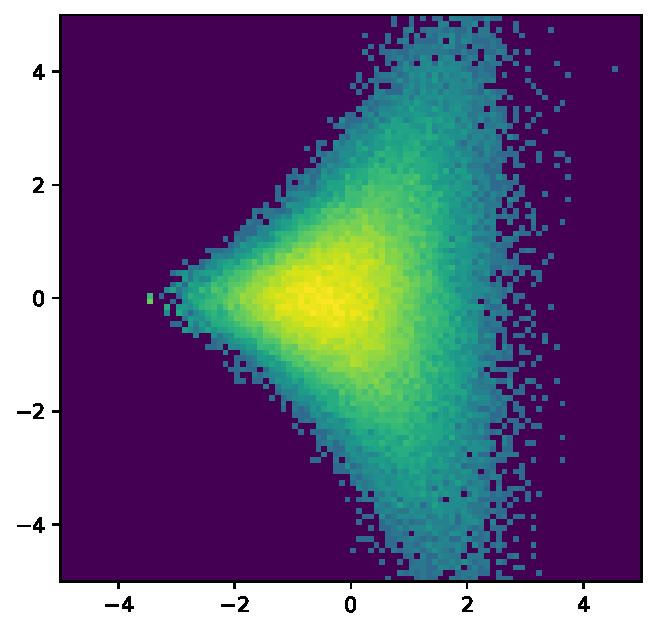
\includegraphics[width=.22\linewidth]{histogram_true_funnel1.pdf}
         &  
          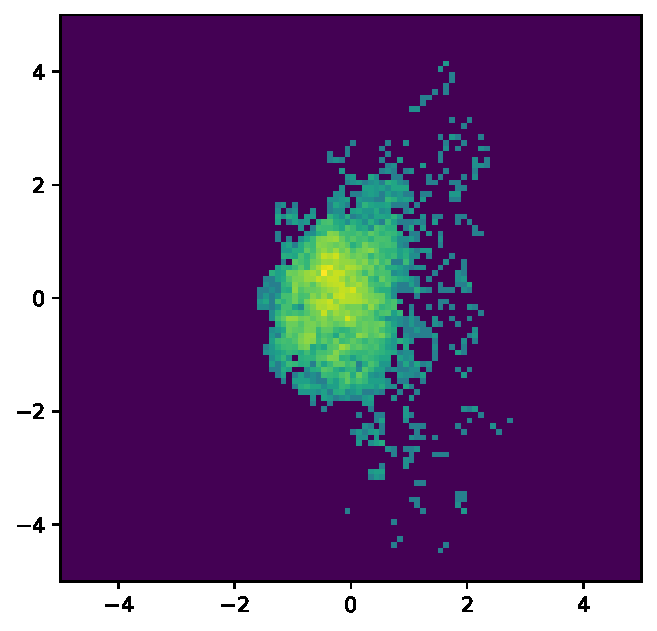
\includegraphics[width=.22\linewidth]{histogram_isir_funnel1.pdf}
          &
           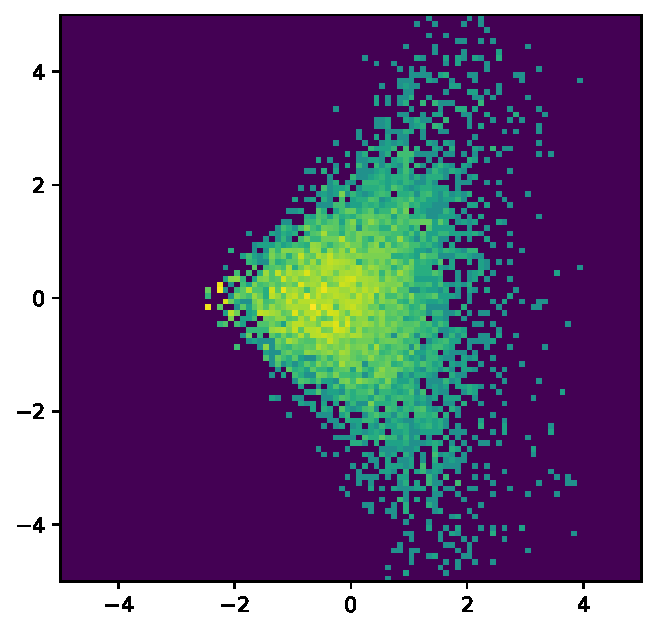
\includegraphics[width=.22\linewidth]{histogram_nuts_funnel1.pdf}
           &
            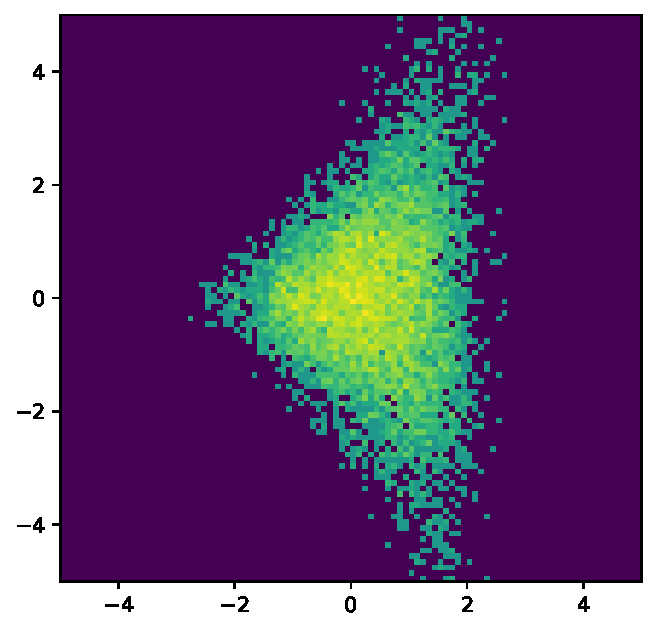
\includegraphics[width=.22\linewidth]{histogram_infine_funnel2.pdf}
    \end{tabular}
\end{figure}
We also present the normalizing constant estimation of this distribution. We initialize the mass matrix and the step-size as discussed previously, and compare IS, AIS, and \InFiNE\ schemes.
The IS estimator is run with $2\cdot 10^5$ samples.
For the \IFIS\ estimator, the number of samples is $N = 2\cdot 10^4$ and the trajectory length is $K=10$. The AIS estimator is run with $2\cdot 10^4$ samples, with the annealing scheme presented in \cite[Section 6.2]{grosse2015sandwiching} of length $K=50$. Moreover, the parameters of the HMC transitions in AIS (mass matrix, step-size) are set to the estimated parameters of the HMC algorithm in Pyro. 
\begin{figure}[!ht]
    \centering
    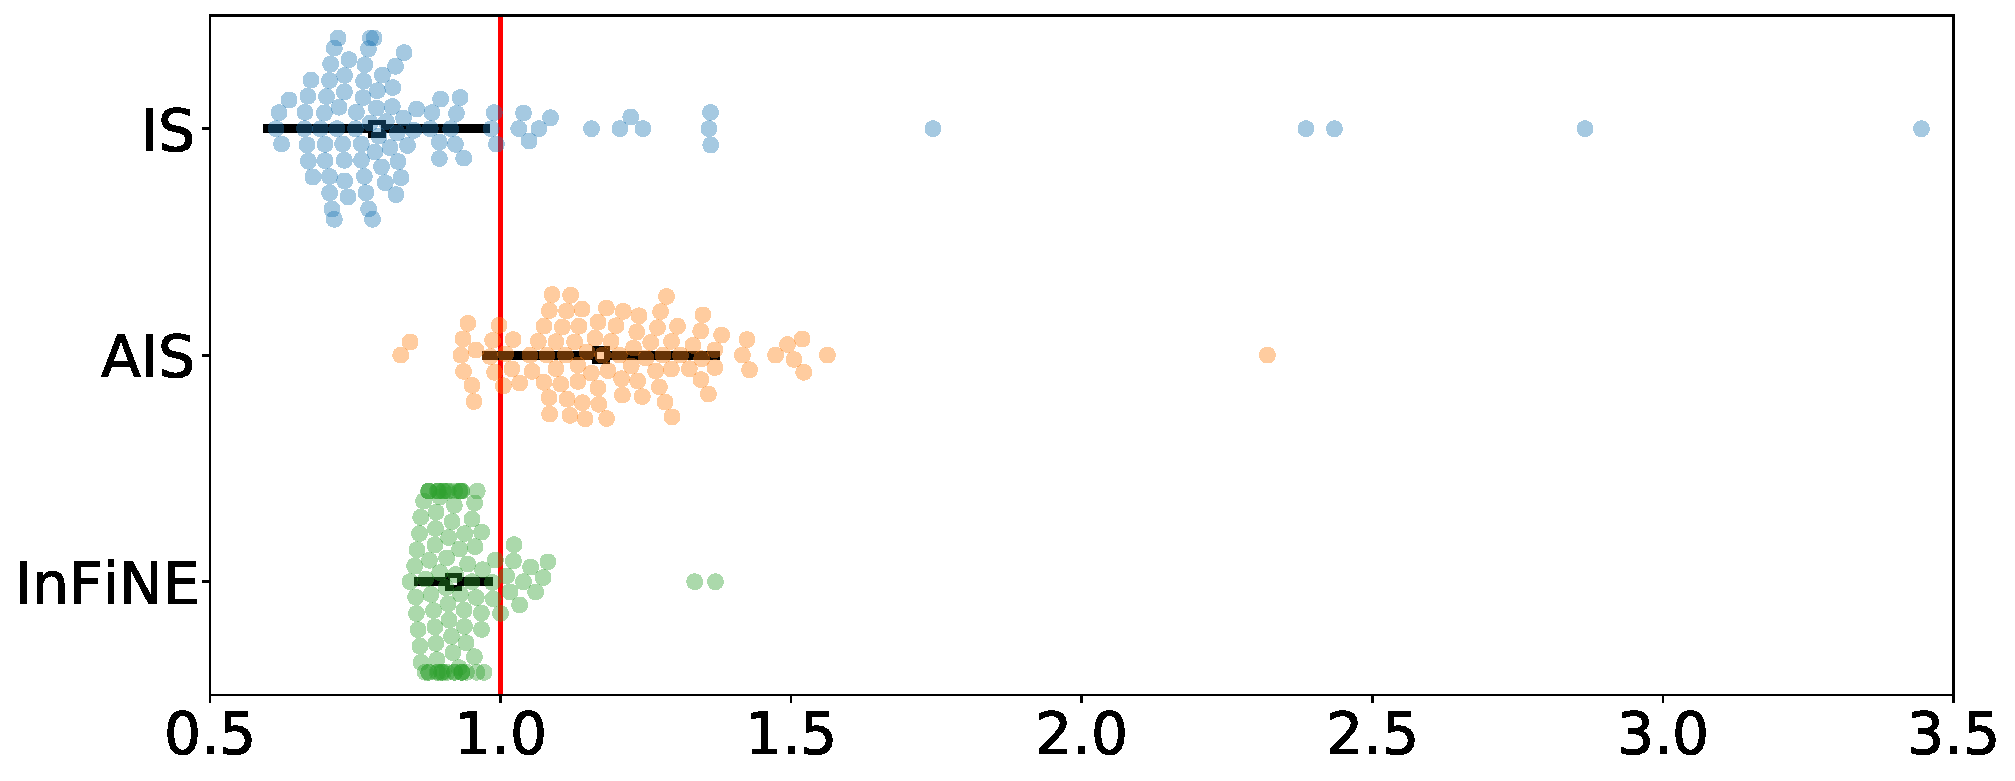
\includegraphics[width=0.7 \linewidth]{funnel.pdf}
    \label{fig:funnel_estimation}
    \caption{200 independent estimations of the normalizing constant of $\pi$. The prior used is a centered Gaussian distribution with $4\mathbf{I}_d$ as covariance matrix. The true value is $Z=1$ (red line). The figure displays the median (square) and the interquartile range (solid lines) in each case.}
\end{figure}


\subsection{VAE experiments}
\label{supsec:vae_exps}
We detail in this section \InFiNE\ VAE with $N$ samples (similarly to the IWAE algorithm). Recall that for each sample,  a trajectory of length $K$ is produced. 
For simplicity, we use $N=1$ in all our experiments to outline \IFIS\ VAE in several experimental settings. It is expected that extension to $N > 1$ will further improve the results.
%Conclusions drawn on the \InFiNE VAE however still hold for the case $N>1$.
Recall that the  lower bound $\elboneq$ is 
\begin{align*}
    \elboneq(\theta, \phi; y) &= \int_{} \proposal_N( \chunku{x}{1}{N})   \log \estConstC{\chunku{x}{1}{N}} \rmd \chunku{x}{1}{N}\eqsp,\\
&= \int_{} \prod_{i=1}^N q_\phi(x^i\mid y)   \log\left( N^{-1}\sum_{i=1}^N\sum_{k=0}^K w_k(x^i) \frac{p_\theta(y, \transfo^k(x^i))}{q_\phi(\transfo^k(x^i)\mid y)}\right)\rmd \chunku{x}{1}{N}\eqsp.
\end{align*}
Assume here that $q_\phi$ is amenable to the reparameterization trick, that is, there exist some diffeomorphism $V_{\phi,y}$ and some fixed pdf $\densgauss$, such that sampling $x\sim q_\phi(\cdot\mid y)$ boils down to sampling $\epsilon\sim\densgauss$ and set $x = V_{\phi,y}(\epsilon)$.
In the particular case where $N=1$, an estimator of the ELBO and of its gradient are given by
\begin{align*}
    &\widehat{\mathcal{L}}_{\IFIS}(\theta, \phi; y) = \log \sum_{k=0}^K w_k(x) \frac{p_\theta(y, \transfo^k(x))}{q_\phi(\transfo^k(x)\mid y)}\eqsp, \eqsp \text{ where } x\sim q_\phi(\cdot\mid y)\eqsp,\\
    &\nabla \widehat{\mathcal{L}}_{\IFIS}(\theta, \phi; y) = \nabla\log \sum_{k=0}^K w_k(V_{\phi,y}(\epsilon)) \frac{p_\theta(y, \transfo^k(V_{\phi,y}(\epsilon)))}{q_\phi(\transfo^k(V_{\phi,y}(\epsilon))\mid y)}\eqsp, \eqsp \text{ where } \epsilon \sim \densgauss\eqsp.
\end{align*}
This is the setting we consider in our experiments. More generally, inspired by the IWAE approach, we can write an estimator of the ELBO and of its gradient as
\begin{align}
\label{eq:gradient_elboneq}
\nonumber
    &\widehat{\mathcal{L}}_{\IFIS} (\theta, \phi; y) = \log\left( N^{-1}\sum_{i=1}^N\sum_{k=0}^K w_k(x^i) \frac{p_\theta(y, \transfo^k(x^i))}{q_\phi(\transfo^k(x^i)\mid y)}\right)\eqsp, \eqsp \text{ where } \chunku{x}{1}{n}\simiid q_\phi(\cdot\mid y)\eqsp,\\
    &\nabla \widehat{\mathcal{L}}_{\IFIS} (\theta, \phi; y) = \sum_{i=1}^N \varpi_i \nabla\log\left( \sum_{k=0}^K w_k(V_{\phi,y}(\epsilon^i)) \frac{p_\theta(y, \transfo^k(V_{\phi,y}(\epsilon^i)))}{q_\phi(\transfo^k(V_{\phi,y}(\epsilon^i))\mid y)}\right)\\
&\hspace{2.6cm}=\sum_{i=1}^N \varpi_i \nabla\log\estConstC{V_{\phi,y}(\epsilon^i)} \eqsp, \eqsp \text{ where } \chunku{\epsilon}{1}{n} \simiid \densgauss\eqsp,
\end{align}
where $\varpi_i = \estConstC{x^i}/(N\estConstC{\chunku{x}{1}{n}})$.
\begin{algorithm}[h]
\label{alg:sup:vae}
\caption{\IFIS\ VAE, trajectory length $K$, and $N$ samples}
\begin{algorithmic}
   \STATE {\bfseries Input:} batch of samples $x$, latent dim $d$.
   \STATE $(\mathbf{\mu}, \log\, \mathbf{\sigma}) \leftarrow EncoderNeuralNet_\phi(x)$.
   \STATE Sample $N$ initial position and momentums: $q_i \sim \mathcal{N}(\mathbf{\mu},\,\operatorname{diag}(\mathbf{\sigma}^{2}))$ and $p_i \sim \mathcal{N}(0, \mathbf{I}_d)$.
   \FOR{$i=1$ {\bfseries to} $N$}
   \STATE Compute $\transfo^k(q_i, p_i)$
   \textit{ This implies forward / backward passes in the decoder to get} $\nabla \log p_\theta(q^k_i)$.
   \STATE Compute $\varpi_i$.
   \ENDFOR
   \STATE Compute the $\ELBO_{\theta, \phi}$ gradient estimator \eqref{eq:gradient_elboneq}.
   \STATE SGD update of parameters $(\theta, \phi)$ using the gradient estimatior.
\end{algorithmic}
\end{algorithm}

\Cref{tab:vae_results} displays the Negative loglikelihood estimates using both IS and \IFIS\ on the FashionMNIST dataset \cite{xiao2017fashion}. The settings are the same than those used in the MNIST experiment. The conclusions are similar:  the \IFIS\ estimate is almost always better than the IS estimate, by a large margin on small dimensions. The InFiNE VAEs are always better than standard VAEs, and better than IWAE with $N=30$ when the dimension of the latent space is small to moderate. When the dimension of the latent space increases ($d=50$), the  performance differences become relatively small.
\begin{table*}[h]
\centering
\caption{NLL estimates for VAE models on FashionMNIST for different latent space dimensions.}
\label{tab:vae_results}
\begin{tabular}{c|c|c||c|c||c|c||c|c|}
\cline{2-9}
 & \multicolumn{2}{c||}{$d = 4$} & \multicolumn{2}{c||}{$d = 8$} & \multicolumn{2}{c||}{$d = 16$} & \multicolumn{2}{c|}{$d = 50$} \\ \hline
\multicolumn{1}{|c|}{model} & IS & \InFiNE  & IS & \InFiNE& IS  & \InFiNE & IS & \InFiNE \\ \hline
\multicolumn{1}{|c|}{VAE} & $240.61$&$240.19$&$235.78$&$235.73$&$235.02$&$234.96$&$234.82$&$234.83$\\ %\hline
\multicolumn{1}{|c|}{IWAE, $N=5$} & $239.66$&$239.27$&$234.05$&$233.98$&$233.12$&$233.12$&$233.52$&$233.46$ \\ %\hline
\multicolumn{1}{|c|}{IWAE, $N=30$} & $239.25$&$238.47$&$233.63$&$233.49$&$233.01$&$232.71$&$232.88$&$232.76$ \\ \hline
\multicolumn{1}{|c|}{\InFiNE\ VAE, $K=3$} & $238.64$&$237.91$&$233.49$&$233.48$&$233.26$&$233.09$&$233.33$&$233.35$ \\ %\hline
\multicolumn{1}{|c|}{\InFiNE\ VAE, $K=10$} & $238.89$&$238.46$&$233.51$&$233.45$&$233.24$&$233.15$&$233.28$&$233.26$ \\ \hline
\end{tabular}
\end{table*}


\section{Connection with Nested sampling}

%%%%%\subsection{Computing Normalizing constant}

We return here to the problem of computing the normalizing constant $\const$ of the target density $\pi(x) =\rho(x)\likelihood(x)/\const$ to point out a simplification induced by our method compared to the method proposed in \cite{rotskoff:vanden-eijden:2019}.
The method proposed in \cite{rotskoff:vanden-eijden:2019} uses the identity
\begin{equation}\label{eq:nesting}    \const=\int \int_{0}^{\infty}\1(\likelihood(x)> \ell)\rho(x) \rmd \ell \rmd x =\int_0^\infty \mathbb{P}_{X\sim\rho}(\likelihood(X)> \ell) \rmd \ell\eqsp,
\end{equation}
which was instrumental in the construction of nested sampling
\cite{skilling2006nested,chopin:robert:2010}. Using identical level sets as \cite{skilling2006nested}, of the form $\mso:=\{x:\likelihood(x)>\ell\}$ with $\ell>0$ and their dissipative Langevin dynamics, \cite[Equation 13]{rotskoff:vanden-eijden:2019} obtain a concise estimator of the volume of these level sets based on the length of the path $(\transfo^k(X^i))_{k\in\mathbb N}$ remaining inside $\mso$. (This estimator is constructed under a uniform prior assumption and continuous-time integrator, but the argument in \cite{rotskoff:vanden-eijden:2019} easily translates to discrete-time.)

Considering instead \IFIS, it provides an approximation of $\mathbb{P}_{X\sim\rho}(\likelihood(X)> \ell)$ for
a fixed $\ell$, but a more efficient resolution is available, which bypasses repeated approximations induced by the quadrature version of both \cite{skilling2006nested,rotskoff:vanden-eijden:2019}. The crux of the improvement is that paths only need be simulated once, using only the stopping time associated with the lowest positive $\ell$ found in early simulations. Integration over the likelihood levels $\ell$ can then be accomplished with no further approximation. Using a single stopping time as indicated earlier, the following is an unbiased estimator of $\PP_{X\sim\rho}(\likelihood(X)> \ell)$ for all values of $\ell$: 
\begin{equation}
\widehat{\PP}_{X\sim\rho}(\likelihood(X)> \ell) =\frac{1}{N} \sum_{i=1}^N 
 \sum_{k=0}^K \indiacc{\likelihood(\transfo^{k}(X^i))> \ell} \w_k(X^i)\eqsp,
 \qquad
X^{i}\stackrel{\text{iid}}{\sim}\rho\eqsp,
\end{equation}
where the weights $\w_k(X^i)$, defined in \eqref{eq:w_k_first_def}, incorporate the stopping times. Integrating the above over $\ell\in\mathbb{R}^+$ as in \eqref{eq:nesting} leads to an estimator of the normalizing constant $\const$:
\begin{align}\label{eq:nolevel}
\widehat{\const}_{X^{1:N}} &=\frac{1}{N}\sum_{i=1}^{N} \sum_{k=0}^{K}  \int_{\mathbb{R}^+} 
 \mathbb{I}(\likelihood(\transfo^{k}(X^i))> \ell) \w_k(X^i) \rmd \ell\nonumber\\
 &= \frac{1}{N}\sum_{i=1}^{N} 
 \sum_{k=0}^K\likelihood(\transfo^k(X^i)) \w_k(x^i)\eqsp,
\end{align}
where we used the slice sampling identity 
\[ 
 \int_{\mathbb{R}^+} \indiacc{\likelihood(\transfo^{k}(x))> \ell} \rmd \ell=\likelihood(\transfo^{k}(x))\eqsp.
\]
In conclusion, the \IFIS~estimator of $\const$ coincides with the conformal Hamiltonian version of nested sampling with the additional benefit of removing the quadrature approximation.
(Note that, as suggested \Cref{remark1}, we could resort to both forward and backward push-forward rather than starting at $k=0$, which could only improve the precision of the estimator \eqref{eq:nolevel}.)


\begin{thebibliography}{50}

\bibitem[Agakov and Barber, 2004]{agakov2004auxiliary}
Agakov, F.~V. and Barber, D. (2004).
\newblock An auxiliary variational method.
\newblock In {\em International Conference on Neural Information Processing},
  pages 561--566. Springer.

\bibitem[Andrieu et~al., 2010]{andrieu2010particle}
Andrieu, C., Doucet, A., and Holenstein, R. (2010).
\newblock Particle {M}arkov chain {M}onte {C}arlo methods.
\newblock {\em Journal of the Royal Statistical Society: Series B (Statistical
  Methodology)}, 72(3):269--342.

\bibitem[Andrieu et~al., 2018]{andrieu2018uniform}
Andrieu, C., Lee, A., Vihola, M., et~al. (2018).
\newblock Uniform ergodicity of the iterated conditional {SMC} and geometric
  ergodicity of particle {G}ibbs samplers.
\newblock {\em Bernoulli}, 24(2):842--872.

\bibitem[Bingham et~al., 2019]{bingham2019pyro}
Bingham, E., Chen, J.~P., Jankowiak, M., Obermeyer, F., Pradhan, N.,
  Karaletsos, T., Singh, R., Szerlip, P., Horsfall, P., and Goodman, N.~D.
  (2019).
\newblock Pyro: Deep universal probabilistic programming.
\newblock {\em The Journal of Machine Learning Research}, 20(1):973--978.

\bibitem[Buchholz et~al., 2021]{buchholz2021adaptive}
Buchholz, A., Chopin, N., Jacob, P.~E., et~al. (2021).
\newblock Adaptive tuning of {H}amiltonian {M}onte {C}arlo within {S}equential
  {M}onte {C}arlo.
\newblock {\em Bayesian Analysis}.

\bibitem[Burda et~al., 2016]{burda:grosse:2015}
Burda, Y., Grosse, R., and Salakhutdinov, R. (2016).
\newblock Importance weighted autoencoders.
\newblock In {\em The 4th International Conference on Learning Representations
  (ICLR)}.

\bibitem[Che et~al., 2020]{che:bengio:2020}
Che, T., Zhang, R., Sohl-Dickstein, J., Larochelle, H., Paull, L., Cao, Y., and
  Bengio, Y. (2020).
\newblock Your {GAN} is secretly an energy-based model and you should use
  discriminator driven latent sampling.
\newblock {\em arXiv preprint arXiv:2003.06060}.

\bibitem[Chen et~al., 2000]{chenetal00}
Chen, M.-H., Shao, Q.-M., and Ibrahim, J.~G. (2000).
\newblock {\em {M}onte {C}arlo Methods in {B}ayesian Computation}.
\newblock Springer-Verlag, New York.

\bibitem[Chib, 1995]{chib:1995}
Chib, S. (1995).
\newblock Marginal likelihood from the {G}ibbs output.
\newblock {\em J. American Stat. Assoc.}, 90:1313--1321.

\bibitem[Chopin and Robert, 2010]{chopin:robert:2010}
Chopin, N. and Robert, C.~P. (2010).
\newblock Properties of nested sampling.
\newblock {\em Biometrika}, 97(3):741--755.

\bibitem[Cremer et~al., 2017]{cremer2017reinterpreting}
Cremer, C., Morris, Q., and Duvenaud, D. (2017).
\newblock Reinterpreting importance-weighted autoencoders.
\newblock {\em arXiv preprint arXiv:1704.02916}.

\bibitem[Cuendet, 2006]{cuendet2006statistical}
Cuendet, M.~A. (2006).
\newblock Statistical mechanical derivation of {J}arzynski’s identity for
  thermostated non-{H}amiltonian dynamics.
\newblock {\em Physical Review Letters}, 96(12):120602.

\bibitem[Del~Moral et~al., 2006]{del2006sequential}
Del~Moral, P., Doucet, A., and Jasra, A. (2006).
\newblock {Sequential Monte Carlo samplers}.
\newblock {\em Journal of the Royal Statistical Society: Series B},
  68(3):411--436.

\bibitem[Ding and Freedman, 2019]{ding2019learning}
Ding, X. and Freedman, D.~J. (2019).
\newblock Learning deep generative models with annealed importance sampling.
\newblock {\em arXiv preprint arXiv:1906.04904}.

\bibitem[Douc et~al., 2018]{douc:moulines:priouret:2018}
Douc, R., Moulines, E., Priouret, P., and Soulier, P. (2018).
\newblock {\em {M}arkov chains}.
\newblock Springer Series in Operations Research and Financial Engineering.
  Springer, Cham.

\bibitem[El~Moselhy and Marzouk, 2012]{el2012bayesian}
El~Moselhy, T.~A. and Marzouk, Y.~M. (2012).
\newblock Bayesian inference with optimal maps.
\newblock {\em Journal of Computational Physics}, 231(23):7815--7850.

\bibitem[Franca et~al., 2019]{francca2019conformal}
Franca, G., Sulam, J., Robinson, D.~P., and Vidal, R. (2019).
\newblock Conformal symplectic and relativistic optimization.
\newblock {\em arXiv preprint arXiv:1903.04100}.

\bibitem[Gelman and Meng, 1998]{gelman1998simulating}
Gelman, A. and Meng, X.-L. (1998).
\newblock Simulating normalizing constants: From importance sampling to bridge
  sampling to path sampling.
\newblock {\em Statistical Science}, pages 163--185.

\bibitem[Geyer, 1993]{geyer:1993}
Geyer, C. (1993).
\newblock Estimating normalizing constants and reweighting mixtures in {M}arkov
  chain {M}onte {C}arlo.
\newblock Technical Report 568, School of Statistics, Univ. of Minnesota.

\bibitem[Grosse et~al., 2015]{grosse2015sandwiching}
Grosse, R.~B., Ghahramani, Z., and Adams, R.~P. (2015).
\newblock Sandwiching the marginal likelihood using bidirectional {M}onte
  {C}arlo.
\newblock {\em arXiv preprint arXiv:1511.02543}.

\bibitem[Gutmann and Hyv\"{a}rinen, 2012]{gutmann:hyvarinen:2012}
Gutmann, M.~U. and Hyv\"{a}rinen, A. (2012).
\newblock Noise-contrastive estimation of unnormalized statistical models, with
  applications to natural image statistics.
\newblock {\em Journal of Machine Learning Research}, 13(1):307--361.

\bibitem[Jarzynski, 2002]{jarzynski2002targeted}
Jarzynski, C. (2002).
\newblock Targeted free energy perturbation.
\newblock {\em Physical Review E}, 65(4):046122.

\bibitem[Jia and Seljak, 2020]{jia2020normalizing}
Jia, H. and Seljak, U. (2020).
\newblock Normalizing constant estimation with {G}aussianized bridge sampling.
\newblock In {\em Symposium on Advances in Approximate Bayesian Inference},
  pages 1--14. PMLR.

\bibitem[Kingma and Welling, 2013]{kingma:welling:2013}
Kingma, D.~P. and Welling, M. (2013).
\newblock Auto-encoding variational {B}ayes.
\newblock {\em arXiv preprint arXiv:1312.6114}.

\bibitem[Kingma and Welling, 2019]{kingma2019introduction}
Kingma, D.~P. and Welling, M. (2019).
\newblock An introduction to variational autoencoders.
\newblock {\em arXiv preprint arXiv:1906.02691}.

\bibitem[Kong et~al., 2003]{kong:etal:2003}
Kong, A., McCullagh, P., Meng, X.-L., Nicolae, D., and Tan, Z. (2003).
\newblock A theory of statistical models for {M}onte {C}arlo integration (with
  discussion).
\newblock {\em Journal of the Royal Statistical Society (Series B)},
  65(3):585--618.

\bibitem[Lawson et~al., 2019]{lawson2019energy}
Lawson, D., Tucker, G., Dai, B., and Ranganath, R. (2019).
\newblock Energy-inspired models: Learning with sampler-induced distributions.
\newblock {\em arXiv preprint arXiv:1910.14265}.

\bibitem[Lindsten et~al., 2015]{lindsten2015uniform}
Lindsten, F., Douc, R., and Moulines, E. (2015).
\newblock Uniform ergodicity of the particle {G}ibbs sampler.
\newblock {\em Scandinavian Journal of Statistics}, 42(3):775--797.

\bibitem[Maddison et~al., 2018]{maddison2018hamiltonian}
Maddison, C.~J., Paulin, D., Teh, Y.~W., O'Donoghue, B., and Doucet, A. (2018).
\newblock Hamiltonian descent methods.
\newblock {\em arXiv preprint arXiv:1809.05042}.

\bibitem[Meng and Schilling, 2002]{meng2002warp}
Meng, X.-L. and Schilling, S. (2002).
\newblock Warp bridge sampling.
\newblock {\em Journal of Computational and Graphical Statistics},
  11(3):552--586.

\bibitem[Mnih and Rezende, 2017]{mnih2016variational}
Mnih, A. and Rezende, D.~J. (2017).
\newblock Variational inference for {M}onte {C}arlo objectives.
\newblock In {\em International Conference on International Conference on
  Machine Learning}, page 2188–2196.

\bibitem[M{\"u}ller et~al., 2019]{muller2018neural}
M{\"u}ller, T., McWilliams, B., Rousselle, F., Gross, M., and Nov{\'a}k, J.
  (2019).
\newblock Neural importance sampling.
\newblock {\em ACM Transactions on Graphics}, 38(145).

\bibitem[Neal, 2001]{neal:2001}
Neal, R.~M. (2001).
\newblock Annealed importance sampling.
\newblock {\em Statistics and Computing}, 11:125--139.

\bibitem[Neal, 2005]{neal2005hamiltonian}
Neal, R.~M. (2005).
\newblock Hamiltonian importance sampling.
\newblock \url{www.cs.toronto.edu/pub/radford/his-talk.ps}.
\newblock Talk presented at the Banff International Research Station (BIRS)
  workshop on Mathematical Issues in Molecular Dynamics.

\bibitem[Newton and Raftery, 1994]{newton:raftery:1994}
Newton, M. and Raftery, A. (1994).
\newblock Approximate {B}ayesian inference by the weighted likelihood bootstrap
  (with discussion).
\newblock {\em Journal of the Royal Statistical Society: Series B (Statistical
  Methodology)}, 56:1--48.

\bibitem[Owen and Zhou, 2000]{owen:zhou:2000}
Owen, A. and Zhou, Y. (2000).
\newblock Safe and effective importance sampling.
\newblock {\em Journal of the American Statistical Association},
  95(449):135--143.

\bibitem[Papamakarios et~al., 2019]{papamakarios2019normalizing}
Papamakarios, G., Nalisnick, E., Rezende, D.~J., Mohamed, S., and
  Lakshminarayanan, B. (2019).
\newblock Normalizing flows for probabilistic modeling and inference.
\newblock {\em arXiv preprint arXiv:1912.02762}.

\bibitem[Prangle, 2019]{prangle2019distilling}
Prangle, D. (2019).
\newblock Distilling importance sampling.
\newblock {\em arXiv preprint arXiv:1910.03632}.

\bibitem[Procacci et~al., 2006]{procacci2006crooks}
Procacci, P., Marsili, S., Barducci, A., Signorini, G.~F., and Chelli, R.
  (2006).
\newblock Crooks equation for steered molecular dynamics using a
  {N}os{\'e}-{H}oover thermostat.
\newblock {\em The Journal of Chemical Physics}, 125(16):164101.

\bibitem[Rotskoff and Vanden-Eijnden, 2019]{rotskoff:vanden-eijden:2019}
Rotskoff, G. and Vanden-Eijnden, E. (2019).
\newblock Dynamical computation of the density of states and {B}ayes factors
  using nonequilibrium importance sampling.
\newblock {\em Physical Review Letters}, 122(15):150602.

\bibitem[Rubin, 1987]{rubin1987comment}
Rubin, D.~B. (1987).
\newblock Comment: A noniterative sampling/importance resampling alternative to
  the data augmentation algorithm for creating a few imputations when fractions
  of missing information are modest: The {SIR} algorithm.
\newblock {\em Journal of the American Statistical Association},
  82(398):542--543.

\bibitem[Ruiz et~al., 2020]{ruiz:titsias:doucet:2020}
Ruiz, F.~J., Titsias, M.~K., Cemgil, T., and Doucet, A. (2020).
\newblock Unbiased gradient estimation for variational auto-encoders using
  coupled {M}arkov chains.
\newblock {\em arXiv preprint arXiv:2010.01845}.

\bibitem[Skilling, 2006]{skilling2006nested}
Skilling, J. (2006).
\newblock Nested sampling for general {B}ayesian computation.
\newblock {\em Bayesian Analysis}, 1(4):833--859.

\bibitem[Smith and Gelfand, 1992]{smith1992bayesian}
Smith, A.~F. and Gelfand, A.~E. (1992).
\newblock Bayesian statistics without tears: a sampling--resampling
  perspective.
\newblock {\em The American Statistician}, 46(2):84--88.

\bibitem[Tjelmeland, 2004]{tjelmeland2004using}
Tjelmeland, H. (2004).
\newblock Using all {M}etropolis--{H}astings proposals to estimate mean values.
\newblock Technical report.

\bibitem[Tokdar and Kass, 2010]{tokdar2010importance}
Tokdar, S.~T. and Kass, R.~E. (2010).
\newblock Importance sampling: a review.
\newblock {\em Wiley Interdisciplinary Reviews: Computational Statistics},
  2(1):54--60.

\bibitem[Turner et~al., 2019]{turner:hung:2019}
Turner, R., Hung, J., Frank, E., Saatchi, Y., and Yosinski, J. (2019).
\newblock Metropolis-{H}astings generative adversarial networks.
\newblock In {\em International Conference on Machine Learning}, pages
  6345--6353. PMLR.

\bibitem[van Dyk and Park, 2008]{vandyk:park:2008}
van Dyk, D.~A. and Park, T. (2008).
\newblock Partially collapsed {G}ibbs samplers.
\newblock {\em Journal of the American Statistical Association},
  103(482):790--796.

\bibitem[Wirnsberger et~al., 2020]{wirnsberger2020targeted}
Wirnsberger, P., Ballard, A.~J., Papamakarios, G., Abercrombie, S.,
  Racani{\`e}re, S., Pritzel, A., Rezende, D.~J., and Blundell, C. (2020).
\newblock Targeted free energy estimation via learned mappings.
\newblock {\em arXiv preprint arXiv:2002.04913}.

\bibitem[Wu et~al., 2016]{wu:burda:grosse:2016}
Wu, Y., Burda, Y., Salakhutdinov, R., and Grosse, R. (2016).
\newblock On the quantitative analysis of decoder-based generative models.
\newblock {\em arXiv preprint arXiv:1611.04273}.

\bibitem[Xiao et~al., 2017]{xiao2017fashion}
Xiao, H., Rasul, K., and Vollgraf, R. (2017).
\newblock Fashion-mnist: a novel image dataset for benchmarking machine
  learning algorithms.
\newblock {\em arXiv preprint arXiv:1708.07747}.

\end{thebibliography}



\end{document}
